\section{\label{sec:RL_theory}Reinforcement learning for optimal quantum control}

%\marin{add discussion at the end of each example on how algorithm generalizes to many-body systems and what the pitfalls are, etc.;
%add clarifications on RL terminology as it is used in the examples;}

In the previous sections, we introduced the concepts of counterdiabatic driving and optimal control. Here we take on a different approach to quantum control using reinforcement learning (RL). We also discuss how ideas from CD driving can be used in combination with RL to control quantum systems, leading to powerful hybrid approaches. While the previous sections would be useful to grasp the overarching theme, the material below can be considered a self-consistent standalone tutorial on reinforcement learning for quantum control. 
\steve{
We begin with a short overview of reinforcement learning, defining the basic notions and concepts, and elaborating on the details behind a simple RL algorithm, cf.~Sec.~\ref{subsec:OC_via_RL}. We then move on to discuss three examples that illustrate some of the features of RL algorithms applied to quantum control: in particular, in Sec.~\ref{sec:RL_1q}, we discuss how to train an RL agent to learn how to prepare a fixed target starting from an arbitrary initial state. Section~\ref{sec:RL_2q} combines ideas from shortcuts to adiabaticity with RL that give rise to hybrid RL/OC algorithms. Finally, in Sec.~\ref{subsec:RL_qubit_ancilla} we discuss how to extract partial information about the state of a controlled qubit with the help of an ancilla to train an RL agent using feedback control.
} 
% \steve{FOR REFERENCE THIS IS FROM THE STA SECTION: We will explicitly consider the control of a simple two level system described by the Landau-Zener model in Sec.~\ref{sec:LandauZener}, which will serve as a paradigmatic example that will also be considered when discussing other the other control techniques that are a focus of this tutorial, namely optimal control in Sec.~\ref{subsec:QOC_example_state} and reinforcement learning in Sec.~\ref{sec:RL_1q} and~\ref{sec:RL_2q}. We will also consider the application of these techniques to simple many-body settings embodied by three variations of the Ising model: (i) nearest neighbor, (ii) infinite range, and (iii) non-integrable.}
% Alternatively, readers not interested in ML methods, can readily skip this section.  \\


Modern machine learning (ML) stands on three pillars~\cite{mehta2019high,carleo2019machine,carrasquilla2020machine,krenn2023artificial}:
(i) \textit{Supervised learning} deals with labeled data, and aims at finding the most probable label for new, unseen datapoints. Notable examples include image recognition or classification tasks based on linear and logistic regression. (ii) The goal of \textit{unsupervised learning}, on the other hand, is to produce an approximate model for the probability distribution that generates a given dataset; once such a model is trained, we can use it to produce more data with the desired properties. This includes, for instance, generative models that can compose music, draw paintings, or write text. (iii) Last, in \textit{reinforcement learning} (RL)~\cite{sutton_barto_rl}, an agent learns to execute a given task by interacting with its environment. 
Note that in RL the term `environment' refers to the physical system the agent interacts with [see Fig.~\ref{fig:RL-scheme}]; this is in contrast to the notion of environment in open systems.
RL is designed for problems that require an interactive feedback loop. The main objective is to learn a strategy (a.k.a.~policy) that, based on observations of the environment, helps the agent manipulate or steer the environment. Reinforcement learning and optimal control share many common features and can be thought of as the two sides of the same coin~\cite{todorov2006optimal}. Therefore, when leveraging ML for quantum control~\cite{ref5, ref6}, RL appears as a natural choice for many (though certainly not all) quantum control setups. 


\begin{figure}[h!]
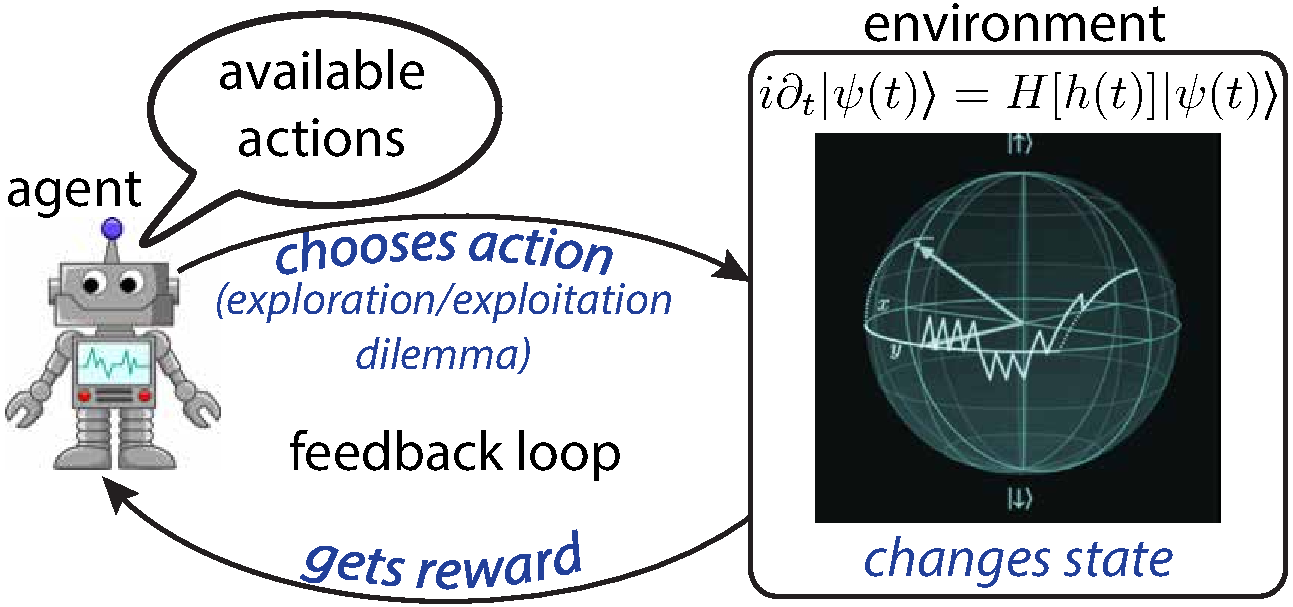
\includegraphics[width=0.4\columnwidth]{RL_image.pdf}
\caption{
RL in a nutshell: the agent observes its environment in a given state, and is presented with a choice of actions to pick from, each of which changes the state of the environment. As a consequence of its decision, the agent is given a reward, depending on the new environment state. Similar to animals being rewarded for achieving a task during training, the goal in RL is to maximize the long-term expected return. This is accomplished through learning about those properties of the environment that are particularly relevant for maximizing the cumulative reward. During the training process, RL agents autonomously figure out an optimal policy to perform the task.
}
\label{fig:RL-scheme}
\end{figure}


\begin{table}[!h]
\centering
\begin{tabular}{|p{12.5cm}|c|}
\hline
Object & Proposed Symbol \\
\hline\hline
states and state space & $s\in\mathbf{S}$ \\
\hline
actions and action space & $a\in\mathbf{A}$ \\
\hline
rewards and reward space & $r\in\mathbf{R}$ \\
\hline
trajectory & $\tau$ \\
\hline
expected return & $\mathbf{G}(\tau)$ \\
\hline
episode length (number of time steps) & $T$ \\
\hline
transition probability & $p(s'|s,a)$ \\
\hline
policy (strategy) & $\pi(a|s)$ \\
\hline
Q function & $Q_\pi(s,a)$ \\
\hline
probability for a trajectory & $P_\pi(\tau)$ \\
\hline
RL objective & $\mathbf{J}$ \\
\hline
variational (learning) parameters & $\theta$ \\
\hline
Monte Carlo samples & $N$ \\
\hline

\hline
\end{tabular}
\caption{Summary of notation for the most common quantities used in RL.}
\label{table:RLSymbols}
\end{table}


In RL, the environment is initialized in a certain state $s_0$, and the agent is presented with a set of actions $\mathbf{A}$ to choose from. Depending on the action $a_t$ selected, the environment reacts and changes state: $s_t\to s_{t+1}$. After each such step $t$, the agent observes the new state of the environment, and is given a reward $r_{t+1}$ that quantifies the quality of the action taken w.r.t.~the objective of the task. Based on this information, the agent then makes an educated guess to select the next action, and so forth, cf.~Fig.~\ref{fig:RL-scheme}. The goal of the agent is to bring the environment into a desired state. To do so, its objective is to maximize the cumulative expected reward $\mathbf{G}$, called return. The expectation is taken over the policy (i.e., the strategy) of the agent and the environment dynamics if the latter is stochastic. Such optimization in expectation brings out as a clear advantage of RL the ability to learn in uncertain or stochastic environments. The learning process in RL is often divided into episodes, which typically comprise a fixed number of steps; once the episode comes to an end, the environment is reset to its initial state $s_0$ and the agent starts over again. Importantly, however, the agent keeps building on the experience gained in previous episodes. 

To select an action, the agent uses a probability distribution $\pi$, called a policy (or strategy). Given a state of the environment, the policy $\pi(a|s)$ defines the probability of taking each of the available actions. If the policy is a delta-function over the actions, we call it deterministic; such a case corresponds to selecting specific actions with certainty, e.g., when applying a fixed external control protocol to the environment. One issue with deterministic policies is that they always produce the same output, and hence the RL agent cannot cause the environment to behave differently, to learn from. To explore new actions (and ultimately determine which one is optimal for the given state), the policy in RL is typically non-deterministic: for instance, if the action space is discrete, one can think of the policy as a normalized state-dependent histogram (distribution) over the available actions; for continuous action spaces, the policy is a continuous probability density, such as a Gaussian or a Lorentzian. However, if the agent explores too much (i.e., its policy is close to a uniform distribution), it cannot learn a better policy either. This tension between exploring new actions and exploiting the already gathered knowledge is known as the `exploration-exploitation dilemma'. 

RL algorithms iteratively improve the policy until it becomes (close to) optimal. Optimal policies, by definition, maximize the total expected return $\mathbf{G}$. In an alternative formulation of the learning procedure, we can look at the state of the environment, and try to predict what the expected return from this state onward (following a fixed policy) should be. This leads us to the concept of action-value (or Q-) functions $Q_\pi(s,a)$; they assign an expected return value to each state-action pair. Once the Q-function is known, one can extract a policy from it by, e.g., looking up the values of different actions for a fixed state, and taking the action that maximizes the action-value function. %\callum{I feel like a lot of important definitions were just introduced, but reading this the first time I am not sure I remembered, e.g., what $\pi$ was by the time I got to the end. I do not have any productive comment on this, just wanted to write this first thought so we can discuss.}

\begin{figure}[h!]
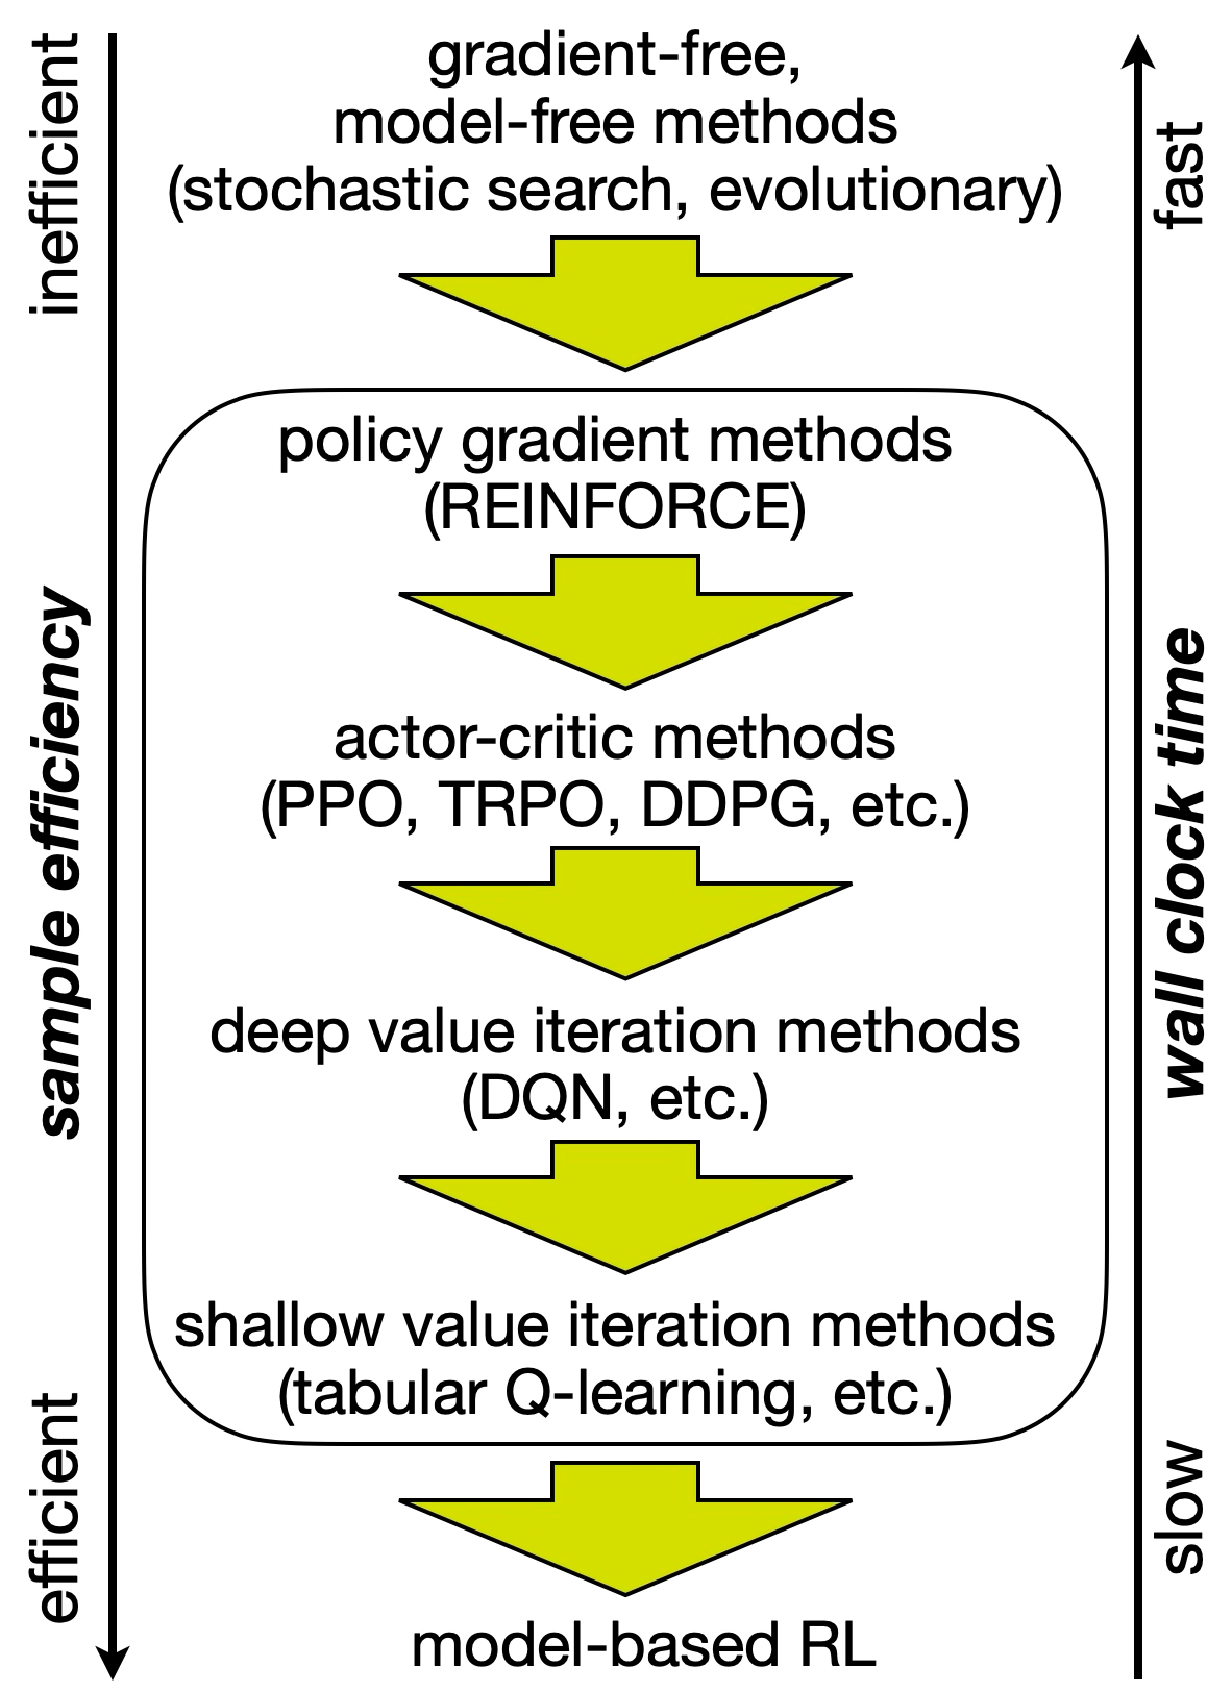
\includegraphics[width=0.3\columnwidth]{RL_sample_efficiency.pdf}
\caption{
Heuristic schematic of sample efficiency and runtime of some RL algorithms.
}
\label{fig:RL_sample_eff}
\end{figure}

Reinforcement learning is not a single algorithm; instead, it should be viewed as a framework that comprises a collection of optimization algorithms, broadly divided into two classes: In policy gradient methods one approximates the policy $\pi\approx\pi_\theta$ with a set of variational parameters $\theta$. For instance, $\theta$ can be the weights and biases of a deep neural network, or $\theta=(\mu,\sigma^2)$ contain the mean and the variance of a Gaussian distribution in the case of continuous actions~\cite{sutton_barto_rl}, but other variational ans\"atze (e.g., a matrix product state or a tensor network more generally~\cite{metz2023self,rose2024combining}) might be better suited to the particular problem at hand. The parameters $\theta$ are then updated using the gradient of the total expected return, estimated, e.g., using Monte Carlo sampling. Examples of widely used algorithms include Policy Gradient (PG)~\cite{williams1992simple}, Proximal Policy Optimization (PPO)~\cite{schulman2017proximal}, Trust-Region Policy Optimization (TRPO)~\cite{schulman2015trust}, and Actor-Critic (AC) methods~\cite{konda1999actor}. Alternatively, Value-Function methods allow us to encode information about the policy; they aim at improving the $Q$-function itself which allows us to indirectly improve the policy~\cite{sutton_barto_rl}. Such methods include, among others, Q-learning~\cite{watkins1992q-learning} and its deep-learning version -- DQN~\cite{mnih2015human}, Deep Deterministic Policy Gradient (DDPG)~\cite{lillicrap2015continuous}, etc. Policy gradient methods are typically less sample-efficient, since updating the policy renders the old data obsolete; thus, new data have to be collected more frequently. Value-function methods, on the other hand, are often off-policy: this feature allows them to learn from old data and makes them more sample efficient. 
Sample efficiency determines the suitability of RL algorithms for quantum control. This is particularly relevant for experimental applications. Depending on the details, collecting rewards from the environment can bring a substantial overhead. In a simulator, if it is easier/faster to generate data than training the agent, Policy Gradient and Actor-Critic algorithms are typically a good starting point. In potential applications to experiments, Deep Q-Learning may be a good choice since it is off-policy. The relative sample efficiency is shown in Fig.~\ref{fig:RL_sample_eff}; the runtime (wallclock time) usually goes in the opposite direction. Deep value iteration methods align with the objective of developing algorithms for both theory and experiment.
Ultimately, which algorithm to use depends on the concrete problem and setup at hand: in some cases, it is easier to learn the policy directly, whereas in others -- the policy may be too complex, but the value function may be easier to approximate.

When it comes to applications of RL for the manipulation of quantum systems, we can broadly identify four mutually overlapping areas: quantum state manipulation, or preparation,~\cite{bukov2018reinforcement,yao2021reinforcement,sivak2022model-free,Porotti2022,metz2023self,reuer2023realizing, XiChenRL1, XiChenRL2, XiChenRL3}, quantum metrology~\cite{MarcoRL1}, quantum gate design~\cite{niu2019universal,dalgaard2020global,baum2021experimental,moro2021quantum,nguyen2023reinforcement}, quantum circuit design~\cite{foesel2021quantum,bolens2021reinforcement,he2021variational,herreramarti2022policy,patel2024curriculum}, and quantum error correction~\cite{foesel2018reinforcement, sweke2020reinforcement, andreasson2019quantum, fitzek2020deep,sivak2023real}. 
Out of these, by far the most common set of problems relates to quantum state manipulation. As exemplified in Sec.~\ref{subsec:OC_via_RL} below, the idea here is to use an RL agent to learn a protocol that transfers the population from an initial to a target state. This has been done extensively for both few-particle and many-body systems, in the context of bosonic, fermionic, and spin systems; RL agents have been shown to perform on par with, or better than, some optimal control algorithms in rugged optimization landscapes. An important concern when applying RL to quantum systems is the lack of accessibility to the exact quantum state (quantum states are unmeasurable mathematical constructs). While this is not an issue when training in simulators, it quickly poses a formidable challenge when applications to real experiments come into sight. For this reason, when applying RL to quantum systems one typically defines the RL state as a set of accessible observables, or a sequence of previously taken actions [cf.~Sec.~\ref{subsec:RL_qubit_ancilla}]. Whereas in many cases RL algorithms work using such partially observable environments, extra care needs to be taken to make sure the learning problem remains well-posed. In turn, the reward function in quantum control problems ranges from maximizing a fidelity (or the negative log-fidelity, in the case of many-body states) through minimizing the energy (as is common when targeting ground states), to optimizing the expectation value of a specific observable; RL agents can also be used to manipulate quantum entanglement~\cite{tashev2024reinforcement}. 

%Expand Hybridization Concepts: Provide concrete examples of combining shortcuts to adiabaticity with reinforcement learning in real-world quantum systems. This will distinguish your tutorial from others that focus on individual techniques.

%The long-term goal for RL in quantum control is the efficient manipulation of highly complex quantum systems in the lab, for which we do not have the exact Hamiltonian (i.e., a model). 
%Few-particle systems and many-body quantum simulators (e.g., cold atoms, trapped ions superconducting qubits, etc.) typically have well-established Hamiltonians and can be used to develop and test the RL algorithms in experiments beyond computer simulations. Once this milestone has been reached, the stage will be set to study the control of quantum materials with complex interactions where no exact model is currently known. \steve{REF COMMENT: the last section was meandering without concrete details. It needs to be tightened up.}




\subsection{\label{subsec:OC_via_RL}Optimal control via policy gradients}

In RL, an agent is confronted with the problem of learning to execute a task by interacting with its environment. The environment is described by a state $s$. The agent observes the state of the environment, and is given a choice of actions $a$ to select from, that alter the state of the environment. The environment can react deterministically or stochastically to these actions, following a set of prescribed rules, the so-called transition probabilities $p(s'|s,a)$, that contain the laws governing the physics of the system. The agent is then given a reward $r(s,a)$, which determines how well it performs on the task. Based on this information, the agent then selects a new action, in an attempt to maximize its total expected return $\mathbf{G}$.
The RL agent selects actions based on its policy $\pi(a|s)$, which defines the probability of choosing action $a$ from state $s$. This is repeated for a fixed number of time steps, $T$, that define a learning episode. The sequence of state-action-reward triples $(s,a,r)$ concatenated over the episode, is called a trajectory $\tau$.

In the following, we will take a look at some simple-to-implement reinforcement learning (RL) algorithms. Let us start by deriving REINFORCE -- the simplest policy gradient algorithm. The reinforcement learning objective $\mathbf{J}$ is to maximize the expected total return, starting from an initial state and taking actions according to the policy $\pi(a|s)$ thereafter. Let us denote the probability for the environment to transition from state $s$ to state $s'$ upon taking action $a$ by $p(s'|s,a)$; for an episode of $T$ steps, denoting the initial state distribution by $p(s_0)$, the probability for the trajectory $\tau = (s_0,a_0,r_1,s_1,a_1,\dots,s_{T-1},a_{T-1},r_T,s_T)$ to occur is given by
\begin{equation}
\label{eq:prob_trajs}
    P_\pi(\tau) = p(s_0)\prod_{t=1}^T \pi(a_t|s_t)p(s_{t+1}|s_t,a_t). 
\end{equation}
The RL objective can be defined formally as
\begin{equation}
\label{eq:RL_obj}
    \mathbf J = \mathbb{E}_{\tau\sim P_\pi} \left[ \mathbf G(\tau) | s_{t=0}=s_0 \right],\qquad \mathbf G(\tau)=\sum_{t=1}^T r(s_t,a_t),
\end{equation}
where $\mathbf G$ is the total return for a fixed trajectory $\tau$. The notation $\mathbb{E}_{\tau\sim P_\pi}$ means that we draw a trajectory $\tau$ according to the probability $P_\pi$; in practice, we do this by sampling the initial state distribution $p(s_0)$ and then the policy $\pi(a|s)$ for each episode step at a time (this is similar to generating runs when playing a video game). The expectation value of the return $\mathbf G(\tau)$ over $P_\pi$ requires a sum over all possible trajectories $\tau$, each weighted by its probability to occur $P_\pi(\tau)$. While this sum can formally be written down, it often contains either exponentially or even infinitely many trajectories. This is similar to the concept of partition functions of Feynman path integrals; we can thus borrow the notation:
\begin{equation}
    \mathbf J = \mathbb{E}_{\tau\sim P_\pi} \left[ \mathbf G(\tau) | s_{t=0}=s_0 \right]
    = \int\mathcal{D}\tau\; P_{\pi}(\tau)\; G(\tau),
\end{equation}
where $\mathcal{D}\tau$ is just a formal notation that allows us to do algebraic manipulations.
Notice that RL is designed to optimize in expectation, which allows it to handle non-differentiable or even discontinuous reward functions $r(s,a)$.  

Policy gradient methods in RL directly approximate the policy $\pi$ using a variational ansatz $\pi_\theta$, parametrized by the unknown parameters $\theta$, $\pi\approx\pi_\theta$. The goal is then to find those optimal parameters $\theta$, which optimize the RL objective $\mathbf J(\theta)$ (think of the agent \steve{that} needs to win the game by maximizing the score). To define an update rule for $\theta$, we may use gradient ascent (or any of its generalizations~\cite{mehta2019high}). This requires us to evaluate the gradient of the RL objective w.r.t.~the parameters $\theta$:
\begin{equation}
\label{eq:nabla_J}
\nabla_\theta \mathbf J(\theta) = \nabla_\theta \mathbb{E}_{\tau\sim P_\pi} \left[ \sum_{t=1}^T r(s_t,a_t) | s_{t=0}=s_0 \right] 
= \nabla_\theta \int\mathcal{D}\tau\; P_{\pi_\theta}(\tau)\; \mathbf G(\tau)
= \int\mathcal{D}\tau\; \nabla_\theta P_{\pi_\theta}(\tau)\; \mathbf G(\tau),
\end{equation}
where we brought the derivative inside the path integral; note that the return $\mathbf G(\tau)$ is independent of $\theta$ and hence it is not affected by the derivative. 

Computing the path integral in Eq.~\eqref{eq:nabla_J} exactly is out of reach because we cannot exhaust the space of all trajectories (similar to the difficulty with computing partition functions in statistical mechanics). In addition, in a model-free setting, we do not know the laws of physics governing the dynamics of the system; as a result, our agent does not have access to the transition probabilities $p(s'|s,a)$. Hence, computing the path integral exactly is not a viable approach. These issues require us to find alternative ways, for instance, by estimating the gradient $\nabla_\theta \mathbf J(\theta)$ from samples. This is feasible because our agent interacts with the environment, and hence we can sample trajectories from it. To this end, we need to write the expression for the gradient $\nabla_\theta \mathbf J(\theta)$ as an expectation value over $P_{\pi_\theta}(\tau)$.
This can be accomplished by using the logarithmic derivative rule $\nabla_\theta P_{\pi_\theta} = P_{\pi_\theta} \nabla_\theta \log P_{\pi_\theta}$ almost everywhere (i.e., up to a set of measure zero), in Eq.~\eqref{eq:nabla_J}:
\begin{equation}
\nabla_\theta \mathbf J(\theta) = \int\mathcal{D}\tau\; \nabla_\theta P_{\pi_\theta}(\tau) \mathbf G(\tau) = \int\mathcal{D}\tau\; P_{\pi_\theta}(\tau)\; \nabla_\theta \log P_{\pi_\theta}(\tau)\; \mathbf G(\tau) = \mathbb{E}_{\tau\sim P_\pi} \left[\nabla_\theta \log P_{\pi_\theta}(\tau)\; \mathbf G(\tau)\right].
\end{equation}

The next step is to evaluate $\nabla_\theta \log P_{\pi_\theta}(\tau)$. Since the initial state distribution and the transition probabilities are independent of $\theta$, using the definition of $P_{\pi_\theta}$ in Eq.~\eqref{eq:prob_trajs}, we have $\nabla_\theta \log P_{\pi_\theta}(\tau) = \nabla_\theta \log \pi_\theta(\tau)$ where $\pi_\theta(\tau) = \prod_{t=1}^T \pi_\theta(a_t|s_t)$. We can therefore use Monte Carlo sampling to estimate the gradients directly from a sample of trajectories $\{\tau_j\}_{j=1}^N$ using the policy $\pi_\theta(\tau)$ (together with the initial state and transition probabilities):
\begin{equation}
\label{eq:RL_grad_sampled}
    \nabla_\theta \mathbf J(\theta) = \mathbb{E}_{\tau\sim P_\pi} \left[\nabla_\theta \log \pi_\theta(\tau)\; \mathbf G(\tau)\right]
    \approx \frac{1}{N}\sum_{j=1}^N \nabla_\theta \log \pi_\theta(\tau_j)\; \mathbf G(\tau_j)
    = \frac{1}{N}\sum_{j=1}^N \left( \sum_{t=1}^T \nabla_\theta \log\pi_\theta(a^j_t|s^j_t) \sum_{t'=1}^T r(a^j_{t'},s^j_{t'}) \right).    
\end{equation}
\steve{Here, we first replace the expectation value over trajectories by its Monte Carlo approximation, $\mathbb{E}_{\tau\sim P_\pi}[\cdot]\approx N^{-1}\sum_{j=1}^N(\cdot)$, where each trajectory $\tau_j$ is drawn from the probability $P_\pi$. Then, in the last equality, we used $\log \pi_\theta(\tau) = \log \prod_{t=1}^T \pi_\theta(a_t|s_t) = \sum_{t=1}^T \log\pi_\theta(a^j_t|s^j_t)$, together with the definition of the total return $\mathbf G(\tau)$ from Eq.~\eqref{eq:RL_obj}.
}

Since, in practice, we always deal with a finite number $N$ of trajectories in our sample, the estimate of the gradient for some parameters $\theta_k$ may have a large variance. To alleviate this issue, we use a two-fold strategy: 
first, notice that the $t'$-sum in Eq.~\eqref{eq:RL_grad_sampled} runs over all time steps $t'=1,\dots,T$; however, only times $t'>t$ should contribute to the gradient since rewards obtained at earlier times $t'<t$ do not affect the action at step $t$. Keeping a smaller number of summands naturally reduces the variance of the estimate.
Second, we introduce a so-called baseline $b=N^{-1}\sum_j \sum_{t'=t}^T r(a^j_{t'}|s^j_{t'})$, defined as the average return over the sample. This so-called centering of the training data is a common trick used in ML.
The PG update then takes the form
\begin{equation}
    \nabla_\theta \mathbf J(\theta)
    \approx \frac{1}{N}\sum_{j=1}^N \sum_{t=1}^T \nabla_\theta \log \pi_\theta(a^j_t|s^j_t) \left[\sum_{t'=t}^T r(a^j_{t'},s^j_{t'}) - b\right].
\end{equation}
One can show that these tricks do not change the expectation value $\nabla_\theta \mathbf J(\theta) = \mathbb{E}_{\tau\sim P_\pi} \left[\nabla_\theta \log \pi_\theta(\tau)\; \mathbf G(\tau)\right]$. The corresponding gradient ascent update rule reads as
\begin{equation}
    \theta \leftarrow \theta + \alpha \nabla_\theta \mathbf J(\theta),
\end{equation}
for some step size (sometimes called a learning rate) $\alpha$. 


\subsection{Examples}

Let us now apply the REINFORCE algorithm to the single-qubit quantum control problem. We will do this in a series of three examples of increasing complexity. 
In Example 1, we consider fully observable qubit control: while this is somewhat unrealistic (as we explain later on), it represents the simplest quantum environment, and we use it to gain intuition about how RL works in practice. 
Subsequently, in Example 2 we use RL in combination with insights from CD driving to design a simple algorithm for variational quantum control. Unlike CD driving, our agent aims at preparing the target only at the final time step. 
Finally, in Example 3 we consider a realistic quantum control problem; in contrast to Example 1, the environment here is stochastic and minimally observable.
\steve{Importantly, as will become clear below, the challenge of applying RL to quantum systems lies with the definition of the RL environment -- the choice of actions, states, and rewards -- rather than with the RL algorithm itself. We therefore place significant focus on discussing how to set up the environment, and refer the interested reader to the accompanying Jupyter notebooks for a practical implementation of the PG algorithm.}

\subsubsection{\label{sec:RL_1q}Example: Universal single-qubit state preparation}

Our goal in this example will be to train an RL agent to learn how to prepare the target state $\ket{\psi_\ast}=(1,0)^t$ starting from any single-qubit initial state $|\psi\rangle$ by using a set of predefined gates.

We begin by defining the qubit environment that models the action of gates on the state of the two-level system (2LS).
The state of a qubit $|\psi\rangle\in\mathbb{C}^2$ is modeled by a two-dimensional complex-valued vector with unit norm: $\langle\psi|\psi\rangle:=\sqrt{|\psi_1|^2+|\psi_2|^2}=1$. Every qubit state is uniquely described by two angles $\theta\in[0,\pi]$ and $\varphi\in[0,2\pi)$:
\begin{eqnarray}
\label{eq:blochsphere_state}
|\psi\rangle=
\begin{pmatrix}
\psi_1 \\ \psi_2
\end{pmatrix}=
\mathrm{e}^{i\alpha}
\begin{pmatrix}
\cos\frac{\theta}{2} \\
\mathrm{e}^{i\varphi}\sin\frac{\theta}{2}
\end{pmatrix}
\end{eqnarray}
The overall phase $\alpha$ of a single quantum state has no physical meaning.
Thus, any \steve{single} qubit state can be pictured as an arrow on the unit sphere (called the Bloch sphere) with spherical coordinates $(\theta,\varphi)$. 

To operate on qubits, we use quantum gates. Quantum gates are represented as unitary transformations $U\in \mathrm{U(2)}$, where $\mathrm{U(2)}$ is the unitary group in two dimensions. Gates act on qubit states by matrix multiplication transforming an input state $|\psi\rangle$ into an output state $|\psi'\rangle$: $|\psi'\rangle=U|\psi\rangle$. For this problem, we consider four gates and their inverses:
\begin{equation}
U_0=\mathds{1},\qquad 
U_x=\mathrm{exp}(-i\delta t \sigma^x/2),\qquad
U_y=\mathrm{exp}(-i\delta t \sigma^y/2),\qquad 
U_z=\mathrm{exp}(-i\delta t \sigma^z/2),
\end{equation}
where $\delta t$ is a fixed time step, $\mathrm{exp}(\cdot)$ is the matrix exponential, 
$\mathds{1}$ is the identity, and we remind that the Pauli matrices are defined
\begin{equation}
\mathds{1}=\begin{pmatrix}
1 & 0 \\ 0 & 1
\end{pmatrix}
,\qquad
\sigma^x=\begin{pmatrix}
0 & 1 \\ 1 & 0
\end{pmatrix}
,\qquad
\sigma^y=\begin{pmatrix}
0 & -i \\ i & 0
\end{pmatrix}
,\ \qquad
\sigma^z=\begin{pmatrix}
1 & 0 \\ 0 & -1
\end{pmatrix}.
\end{equation}
We also allow our RL agent to use the inverse operations for $U_x^\dagger, U_y^\dagger, U_z^\dagger$. 

To determine if a qubit, described by the state $|\psi\rangle$, is in a desired target state $|\psi_\ast\rangle$, we compute the fidelity

\begin{eqnarray}
\mathcal F=|\langle\psi_\ast|\psi\rangle|^2\in[0,1].
\end{eqnarray} 
Physically \steve{for a single qubit}, the fidelity corresponds to the angle between the arrows representing the state on the Bloch sphere (we want to maximize the fidelity but minimize the angle between the states).

Now, let us define an episodic RL environment, which contains the laws of physics that govern the dynamics of the qubit (i.e., the application of the gate operations to the qubit state). \steve{We recall that the environment in RL is different from the notion of environment in open systems.} Our RL agent will interact with this environment \steve{by taking actions and observing its states} to learn how to control the qubit to bring it from an initial state to a prescribed target state. To this end, we define the RL states $s=(\theta,\varphi)$ as an array containing the Bloch sphere angles of the quantum state. For each step within an episode, the agent can choose to apply one out of the actions, corresponding to the seven gates $(\mathds{1},U_x,U_y,U_z,U_x^\dagger,U_y^\dagger,U_z^\dagger)$. We use the instantaneous fidelity w.r.t.~the target state as a reward: $r_t=\mathcal F=|\langle\psi_\ast|\psi(t)\rangle|^2$. More formally, we have to define: 
\begin{itemize}

    \item \textbf{State space:} $\mathbf{S} = \{(\theta,\varphi)\;|\;\theta\in[0,\pi],\varphi\in[0,2\pi)\}$. There are no well-defined states to terminate episodes in this task. Instead, we consider a fixed number of time steps $T$, after which the episode terminates deterministically. The target state (i.e., the qubit state we want to prepare) is $|\psi_\ast\rangle=(1,0)^t$: it has the Bloch sphere coordinates $s_\ast=(0,0)$. 

    \item \textbf{Action space:} $\mathbf{A} = \{\boldsymbol{1},U_x,U_y,U_z,U_x^\dagger,U_y^\dagger,U_z^\dagger\}$. Actions \steve{change the state of the controlled system; they} act on RL states as follows: 
    \begin{enumerate}
        \item if the current state is $s=(\theta,\varphi)$, we first create the quantum state $|\psi(s)\rangle$; 
        \item we apply the gate $U_a$ corresponding to action $a$ to the quantum state, and obtain the new quantum state $|\psi(s')\rangle = U_a|\psi(s)\rangle$. 
        \item last, we compute the Bloch sphere coordinates which define the next state $s'=(\theta',\varphi')$, using the Bloch sphere parametrization for qubits given in Eq.~\eqref{eq:blochsphere_state}.
    Note that all actions are allowed from every state. 
    \end{enumerate}

    \item \textbf{Reward space:} $\mathbf{R}=[0,1]$. We use the fidelity between the next state $s'$ and the target state $s_\ast$ as a reward at every episode step: 
    \begin{equation}
        r(s,s',a)= \mathcal F = |\langle\psi_\ast|U_a|\psi(s)\rangle|^2=|\langle\psi_\ast|\psi(s')\rangle|^2
    \end{equation}
    for all states $s,s'\in\mathcal{S}$ and actions $a\in\mathbf{A}$. \steve{This choice is motivated by the fact that the fidelity of the instantaneous state with the target state is a measure of the distance between the states. Alternatively, one can use other reward functions, such as the ground state expectation of the parent Hamiltonian for the target state.}
\end{itemize}

\begin{figure}[t!]
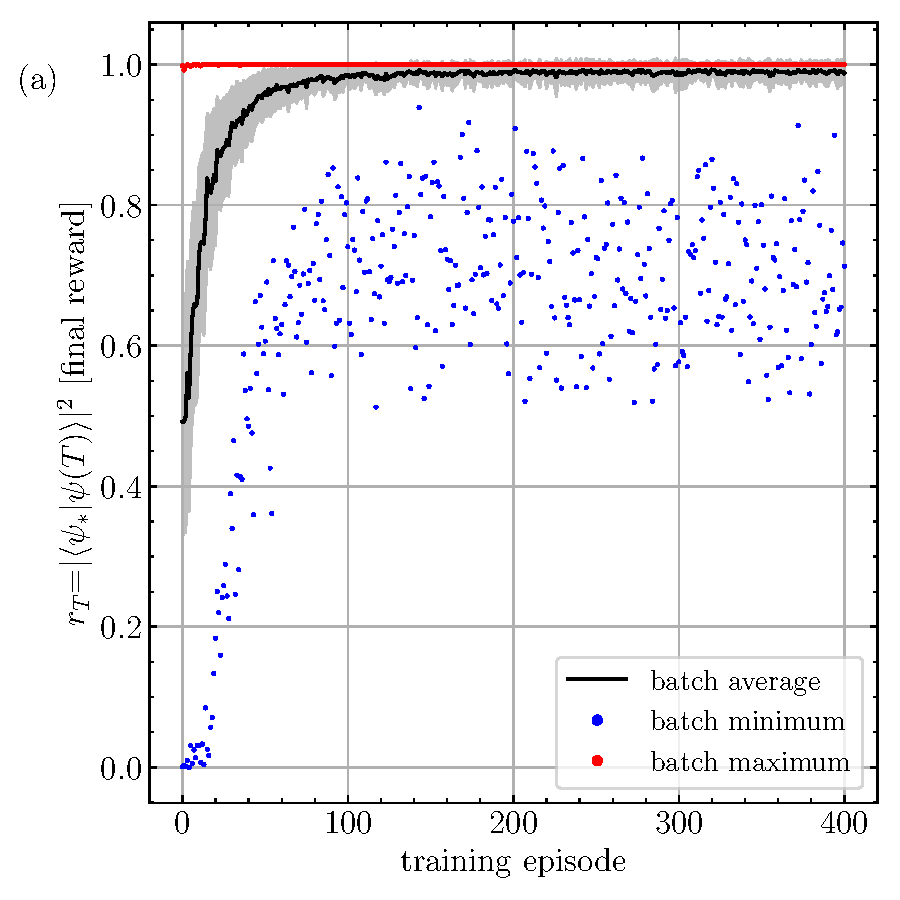
\includegraphics[width=0.45\columnwidth]{RL-1q_training-curve.pdf}
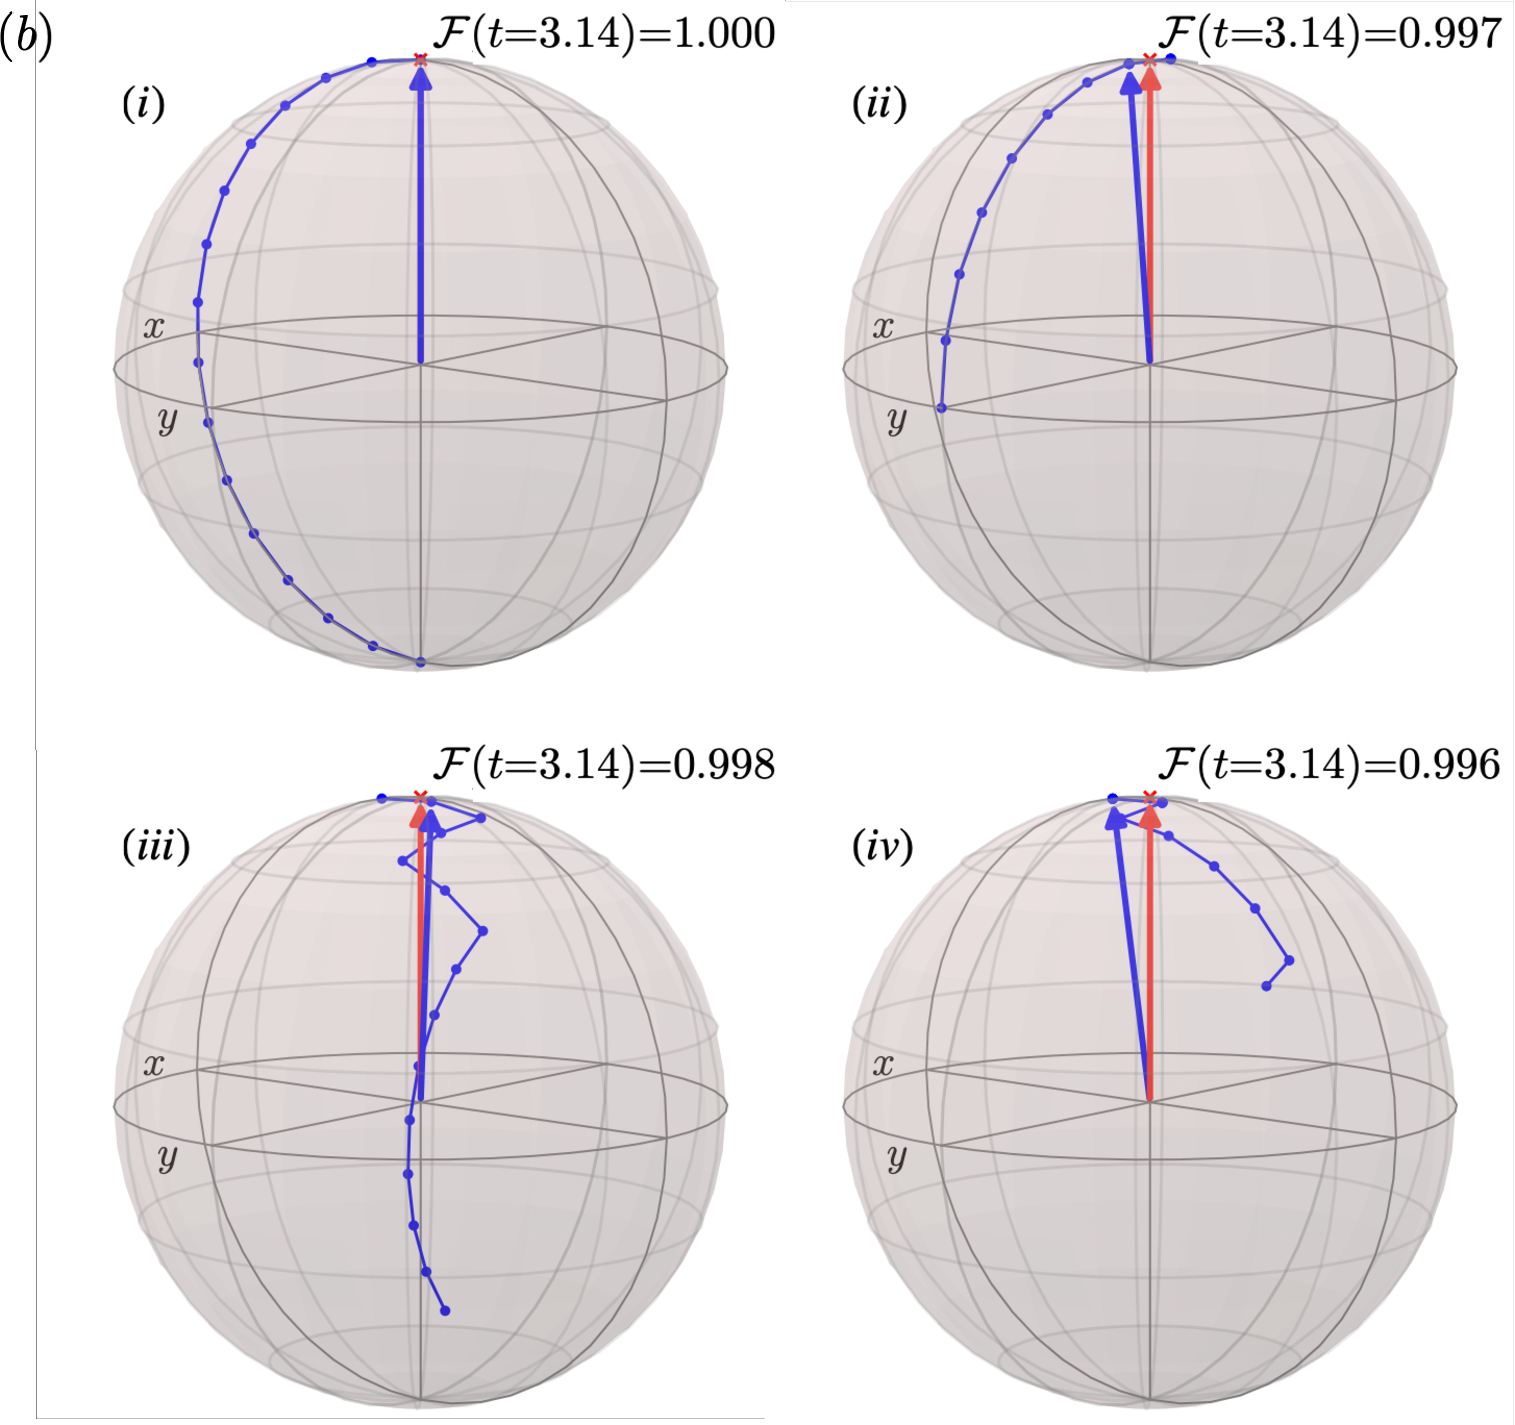
\includegraphics[width=0.45\columnwidth]{RL_1q_init_states.pdf}
\caption{
Universal single-qubit control using reinforcement learning:
\textbf{(a)} training curves for an RL agent learning to prepare the target $|\uparrow\rangle$ states (north pole of Bloch sphere) starting from any initial state. The final reward at the end of the protocol is shown, averaged over a batch of $N=256$ random initial states (black), as well as the minimum/worst-case (blue dashed) and the maximum (red dashed) values within the batch. 
\textbf{(b)} (i-iv) trajectories learned by the RL agent for four different initial states; the target (final) state is shown in red (blue). The agent achieves a fidelity $1-\mathcal{F}$ within the $1\%$ error range. 
We used a fully connected neural network with $(512, 256,7)$ neurons in each layer to learn the optimal strategy using the Policy Gradient algorithm.
The time step is $\delta t = T/\pi$ for a total of $T=15$ time steps.}
\label{fig:RL_qubit}
\end{figure}


Figure~\ref{fig:RL_qubit}(a) shows the result of the training procedure. We use a uniform initial state distribution $p(s_0)$ \steve{since this will expose the agent to a sample of the entire single-qubit Hilbert space; in turn, this will help it learn how to steer any initial state into the target}. To train the agent, we employ the REINFORCE algorithm with a batch of $N=256$ trajectories; \steve{we invite the interested reader to explore the accompanying Jupyter notebook. To this end, the agent runs a large number of episodes during which it explores the control protocol space by taking actions}. The reward at the end of the episode $r_T=|\langle\psi_\ast|\psi(T)\rangle|^2$ tells us how close the final state is to the target. Monitoring this quantity as a function of the training episodes (i.e., iterations of the algorithm) shows a steady increase of the batch average (black solid line) to a value close to unity. For comparison, we also show the best (red) and worst (blue) trajectories from the batch. The spread in the worst trajectories, as training progresses, comes from exploration: the RL agent takes actions probabilistically, and hence occasionally, suboptimal actions can be taken. 

To test the performance of the trained agent, we consider a greedy policy that takes the action with the highest probability deterministically. Figure~\ref{fig:RL_qubit}(b) shows the Bloch sphere trajectories of qubits controlled by the trained RL agent, starting from four different initial states (the time discretization is marked by the blue dots on the trajectory); the target state is shown in as a red arrow, and the final state in blue. \steve{Importantly, we emphasize that there is no further optimization required: once the training process has completed successfully, the same agent knows how to produce the optimal protocol starting from any initial state. This is a prime example of the learning (or generalization) capabilities of RL agents, which contrasts RL from optimal control.} In all cases, the agent manages to bring the state close to the target; the small leftover deviation is caused by the finite timestep $\delta t$. 
Supplementary movies show the trajectories in time.
We invite the interested reader to check out the accompanying Jupyter notebook and explore the behavior of the agent further~\cite{github_code}.

\steve{The example above serves as a stepping stone to learn how RL works in practice. In principle, all one has to do to control more complex quantum systems is redefine the environment, and the same implementation of the RL algorithm can be re-used. However, for quantum many-body systems, this is a tricky task: for instance, there is no convenient Bloch sphere representation for the quantum states. In this case, one can resort to using the bare wavefunction amplitudes, or other exact representations of the state (e.g., different momentum modes in cases, such as the transverse-field Ising model, where the problem can be mapped to a free system, or Clifford tableaus for Clifford circuit dynamics, etc.). One may also resort to suitable approximations, e.g., matrix product states~\cite{metz2023self} whenever appropriate.
We should also point out that the fidelity is typically exponentially small (in the number of qubits) for many-body states; in this case, one typically resorts to minimizing the energy of a parent Hamiltonian (i.e., a Hamiltonian whose ground state is the target state)~\cite{yao2021reinforcement}. It is important to keep in mind that, while RL provides a way to finding optimal protocols for quantum systems, it does not resolve any of the problems of many-body physics associated with representing quantum states or extracting information from them.  
}


\subsubsection{\label{sec:RL_2q}Example: RL vs.~counter-diabatic driving in the presence of trotterization errors}


We now build on the example above and apply RL to the problem of preparing the ground state of a target single-qubit Hamiltonian. We adopt a hybrid approach where the structure of the control terms in the Hamiltonian are designed using knowledge from CD driving (Sec.~\ref{sec:CD}).
In particular, we compare and contrast the behavior of the RL agent to counterdiabatic (CD) driving. Before we dive into the RL implementation, let us briefly mention that CD driving can be enhanced using other ML techniques, see, e.g., Ref.~\cite{ferrer2023physics}. 

As we have seen in Sec.~\ref{sec:STA}, CD driving introduces additional control terms to suppress excitations during the protocol: 
%\marin{fix notation in notebook!}
\begin{equation}
\label{eq:RL_HCD}
    H_\text{CD}(t) = \Delta\sigma^x + \nu(t)\sigma^z - \frac{1}{2}\frac{\Delta\; \dot\nu(t)}{\Delta^2 + \nu^2(t)}\sigma^y.
\end{equation}
As a result, evolving an eigenstate of the initial Hamiltonian $H(0)=\Delta\sigma^x+\nu(0)\sigma^z$ in time with $H_\text{CD}(t)$, the system follows the instantaneous eigenstates of the Hamiltonian $H(t)$ at all times. 
%\steve{REF COMMENT: Explain more the ML terminology ``episode" and ``action space". This reads like an intro to quantum for ML experts but you are much more likely to have an audience of quantum experts wanting to learn ML.}

We now initialize the system in the ground state of the Hamiltonian $H(0)$ at $\nu(0)=\nu_i=+2\Delta$, and want to transfer the population in the ground state at $H(t_\ast)$ at $\nu(t_\ast)=\nu_\ast=-2\Delta$ in a finite amount of time $T$ (referred to as the duration of the protocol). During the evolution, the system is subject to the Hamitlnoan
\begin{equation}
\label{eq:Hg}
    H_g(t) = \Delta\sigma^x + \nu(t)\sigma^z - g(t)\sigma^y,
\end{equation}
where $\nu(t) = (\nu_\ast-\nu_i)t/T + \nu_i$ is a linear drift term that is always kept on (and the RL agent has no control over it), while $g(t)$ is the unknown counter protocol that we want our RL agent to find. The form of the Hamiltonian $H_g(t)$ is motivated by the CD Hamiltonian in Eq.~\eqref{eq:RL_HCD}; however, we do not make any assumptions on the structure of the drive protocol $g(t)$ whatsoever, and we leave it to the RL agent to find its shape.

The qubit evolves following $H_g(t)$, and its state at time $t$ is determined by the time evolution operator, which can be expressed in terms of the time-ordered exponential of the Hamiltonian $H_g(t)$ generating the dynamics:
\begin{equation}
    |\psi(t)\rangle =U(T,0)|\psi(0)\rangle = \mathcal{T}\exp\left(-i \int^t_0\mathrm ds\;  H_g(s)\right)|\psi(0)\rangle .
\end{equation}
Once again, we use the fidelity to determine if a qubit, described by the state $|\psi(t)\rangle$, is in a desired target state $|\psi_\ast\rangle$:
\begin{eqnarray}
    \mathcal F=|\langle\psi_\ast|\psi(t)\rangle|^2 ,\qquad \mathcal F\in[0,1]\; .
\end{eqnarray}

\steve{Now that we have defined the control problem, we discuss how to phrase it within the RL framework. Similar to the example in Sec.~\ref{sec:RL_1q}, we define an episodic RL environment, which contains the laws of physics that govern the dynamics of the qubit (i.e., the time evolution following the Hamiltonian $H_g(t)$). The environment will provide data for the RL agent to learn how to bring the qubit to the target ground state. 
To this end, we discretize the protocol into $N_T$ time steps of size $t$, so that the total duration is $T=N_T\delta t$. At each step, the RL agent constructs the value of the control protocol by selecting an action out of the available action set. The total number of timesteps in the protocol comprises a learning episode. Once an episode comes to an end, the environment is reset to its initial state, and the agent starts constructing the protocol again. In each subsequent episode, the agent uses the knowledge gained during previous protocols. 
}

Now, for each timestep of size $\delta t$ within the episode, the agent has to determine the optimal value of the protocol function $g(t)$; to this end, starting from some initial value $g_i$, we let the agent find the optimal relative change in the protocol (i.e., by how much the protocol value has to change at the given timestep). In practice, we define a minimum protocol size $\delta g$, and consider $2n+1$ steps of size $-n\delta g, -(n-1)\delta g, \dots, -\delta g, 0,\delta g,\dots, (n-1)\delta g, n\delta g$ that the agent has to choose from. We also set $g_i=\frac{1}{2}\frac{\Delta\; \dot\nu(0)}{\Delta^2 + \nu^2(0)}$, which fits our goal to directly compare the performance of the agent with CD driving, cf.~Eq.~\eqref{eq:Hg}.   



\begin{itemize}
    \item \textbf{state space:} $\mathbf{S} = \{(\theta,\varphi)\;|\;\theta\in[0,\pi],\varphi\in[0,2\pi)\}$. There are no well-defined terminal states in this task. Instead, we consider a fixed number of time steps, after which the episode terminates deterministically. 

    \item \textbf{action space:} $\mathbf{A} = \{-n,-(n-1),\cdots,-1,0,1,\cdots,n-1,n\}$. Actions correspond to fixed discrete amounts by which the agent can change the protocol $g(t)$ (see above). Actions act on RL states as follows:
    \begin{enumerate}
        \item if the state at time step $n$ (corresponding to physical time is $t=n\delta t$) is $s=(\theta,\varphi)$, we first create the quantum state $|\psi(s)\rangle$; 

        \item we apply to the quantum state the unitary $U_a$ corresponding to action $a\in\mathbf{A}$, defined by:
            \begin{equation}
                 U_a = \exp(-i \delta t H_{a\times\delta g}(n\delta t)),\qquad 
                 H_{a\delta g}(n\delta t) = \Delta\sigma^x + \nu(n\delta t)\sigma^z - a\delta g\sigma^y,
            \end{equation}
        where $n$ labels the time steps, and $\delta g$ ($\delta t$) is a fixed minimum protocol (time) step size (parameters of our choice). 

        \item we obtain the new quantum state $|\psi(s')\rangle = U_a|\psi(s)\rangle$. 

        \item last, we compute the Bloch sphere coordinates which define the next state $s'=(\theta',\varphi')$, using the Bloch sphere parametrization for qubits given above.
        Note that all actions are allowed from every state. 
    \end{enumerate}

    \item \textbf{reward space:} $\mathbf{R}=[0,+\infty)$. 
    Since we want to incentivize the agent to prepare the target state at the end of the protocol, the reward is given only at the end of the episode. Note the difference to CD driving, where the system is in the instantaneous ground state at any given time during the protocol. In general, such reward functions are referred to as sparse rewards in RL. The return $\mathbf G=r_T$ is then equal to the final reward. 
    %\pablo{I find the reference to measurements a bit distracting; for instance, it makes me wonder why this argument was not made in the previous example. I suggest saying that what you are doing here with the sparse rewards is a different approach to defining the reward space, which could be inspired / justified by the fact that in actual experiments we don't have access to instantaneous fidelity without destroying the state.}
    % I added one paragraph before Example 1 to explain the flow; I also changed the motivation above so it is less confusing; hope it's fine now but let me know if it isn't
    
    Thus, the reward is zero at each step during the protocol: $r_{t<T}=0$, except at the last step, where we use the fidelity between the final state $|\psi(T)\rangle$ and the target state $|\psi_\ast\rangle$ as a reward at the end of every protocol: 

    \begin{equation}
    r(s,s',a)= r_t=
    \left\{\begin{array}{lr}
        0, & \text{for}\qquad t<T\\
        -\log_{10}\left(1-\mathcal F\right), & \text{for}\quad t=T
        \end{array}\right.
    ,\qquad \mathcal F=|\langle\psi_\ast|\psi(T)\rangle|^2,\quad |\psi(T)\rangle = U(T,0)|\psi(0)\rangle,
    \end{equation}
    for all states $s,s'\in\mathbf{S}$ and actions $a\in\mathbf{A}$. 

    Since we are interested in high-fidelity protocols, it is important to build a high resolution into the reward signal. One way to do this is to use the logarithmic fidelity $1-\mathcal{F}$ w.r.t.~the target state at the end of the protocol as a reward. The logarithm allows us to learn on a logarithmic scale. Using a base-$10$ logarithm allows us to interpret the reward as the number of decimal places in the deviation of the fidelity from unity: e.g., $r_t=1$ corresponds to $\mathcal F=0.9$, while $r_t=2$ is equivalent to $\mathcal F=0.99$, etc.

\end{itemize}


\begin{figure}[t]
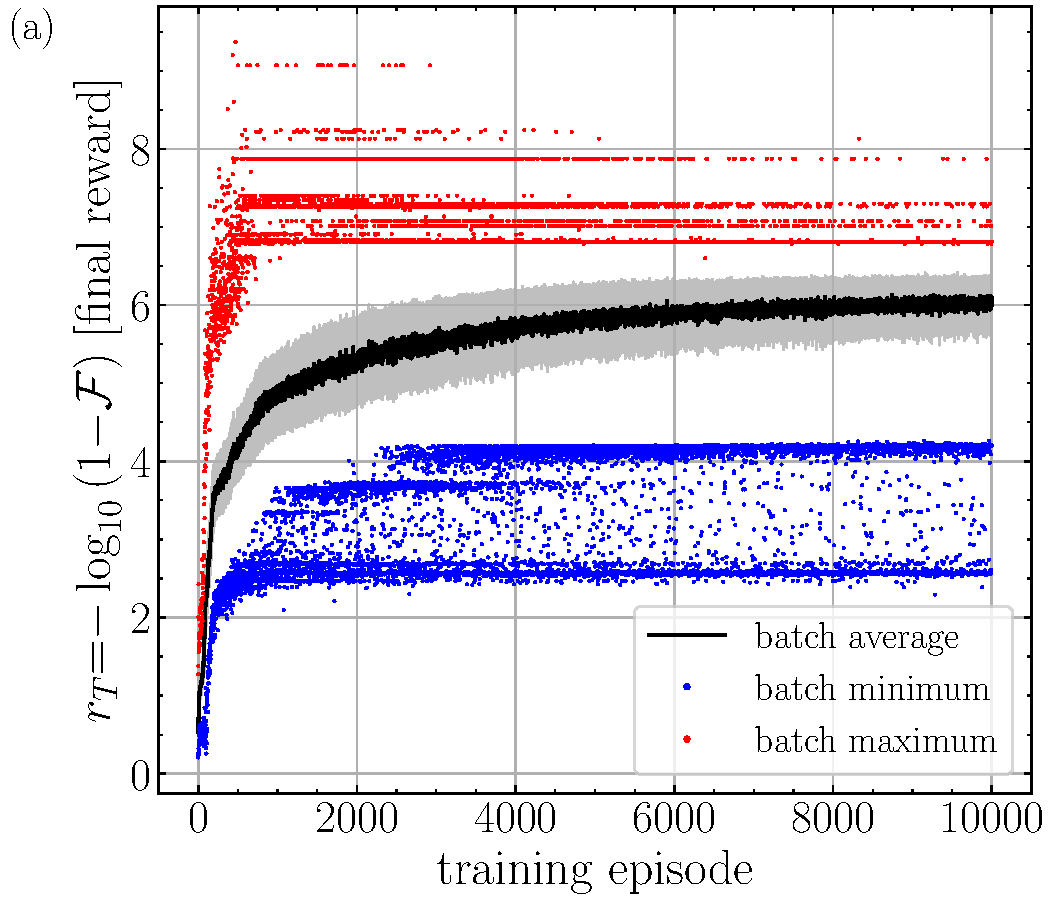
\includegraphics[width=0.33\columnwidth]{PG-STA_training-curve.pdf}
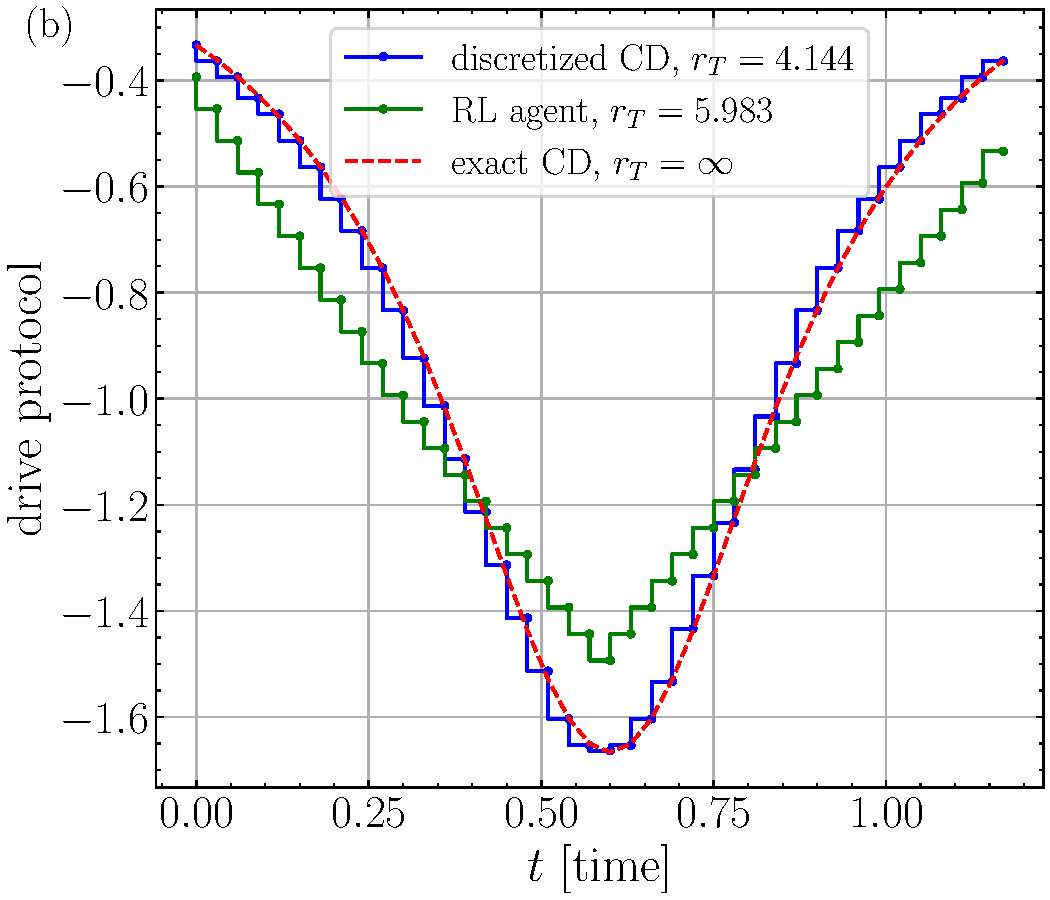
\includegraphics[width=0.33\columnwidth]{PG-STA_protocols.pdf}
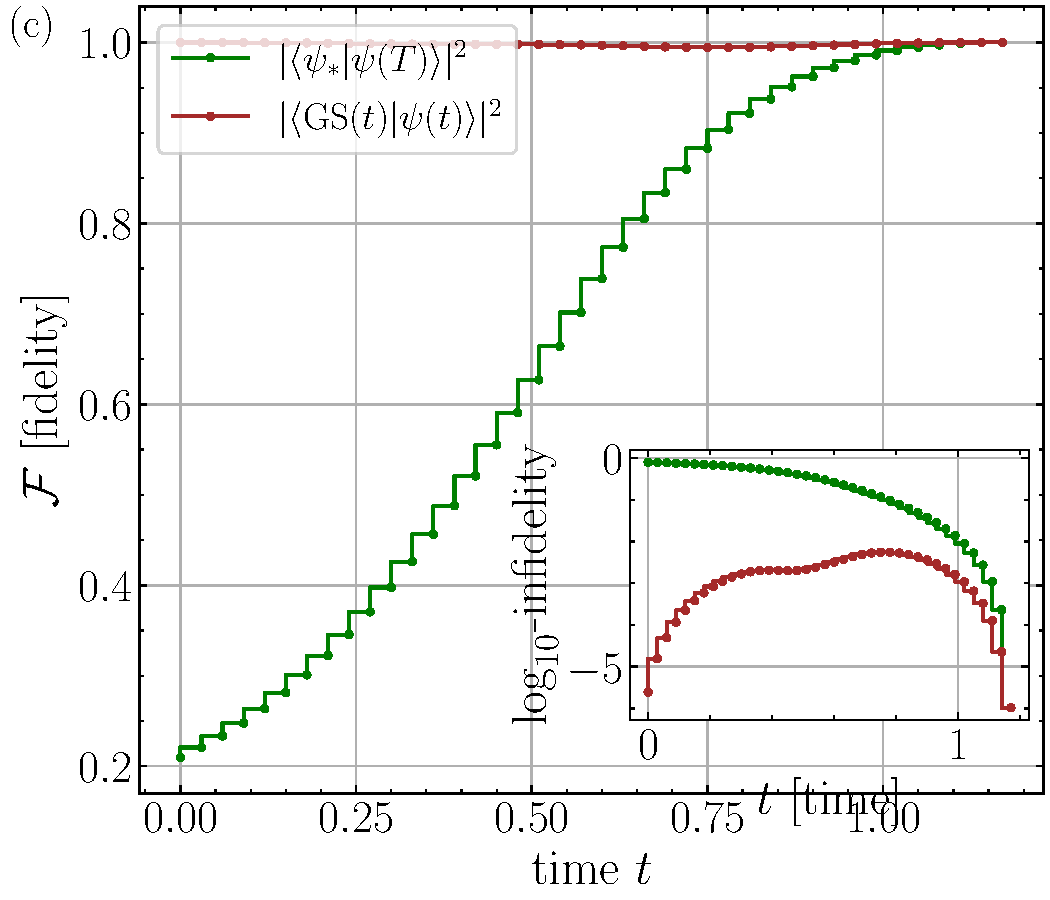
\includegraphics[width=0.33\columnwidth]{PG-STA_fidelity.pdf}
\caption{
Reinforcement learning the CD control problem. 
\textbf{(a)} reward (logarithmic fidelity) at the end of the protocol against the number of training iterations (episodes): training is performed using a batch size of $256$. RL agent achieves an average fidelity $1-\mathcal{F}$ of about $10^{-6}$ (black line, with the shaded area showing the standard deviation); worst (best) protocols in the batch are shown in blue (red). 
\textbf{(b)} comparison of protocols and their final reward (corresponding to the number of decimals in $1-\mathcal{F}$). The exact continuous CD protocol (dashed red) performs worse than the RL agent (green) when time is discretized (blue).
\textbf{(c)} main plot shows the fidelity of the protocol learned by the RL agent (green) and the instantaneous fidelity (brown); inset shows the corresponding infidelities on a logarithmic scale.
}
\label{fig:RL-CD}
\end{figure}

We now apply the REINFORCE algorithm to this RL problem.
Figure~\ref{fig:RL-CD}(a) shows the training curves for the reward $r_T$ at the end of the episode (equal to the total return in this case). Like before, we consider the batch average (black), and the best (red) / worst (blue) protocols within the batch. Notice that achieving a 6-digit reward (i.e., a fidelity of $\mathcal F=0.999999$) requires about $8\times 10^3$ training episodes. We also see that there exist protocols with $r_T>8$ which the agent encounters during the exploration but fails to learn; this can be due to various reasons, e.g., the corresponding protocols may be unstable to small perturbations (recall that the agent takes actions probabilistically), or they may correspond to very deep and isolated minima of the control landscape (and hence, they are difficult to encounter often enough for the signal to accumulate and lead to stable learning).   

Figure~\ref{fig:RL-CD}(b) shows a comparison between the exact CD protocol (red dashed line), its discretization with the environment time step $\delta t$ (blue), and the protocol learned by the RL agent (green). Note that, while the continuous CD protocol is by construction perfect ($r_T=\infty)$, its discretized version has a reduced logarithmic fidelity $1-\mathcal{F}$ of $r_T=4.144$. For comparison, the RL agent achieves $r_T=5.983$. The RL agent achieves a better result, since it optimizes for preparing the target ground state only and pays no attention to the intermediate states of the system, see deviation from unity in the overlap with the instantaneous ground state (brown curve in Fig.~\ref{fig:RL-CD}(c)). By contrast, exact CD driving keeps the system in the instantaneous GS of $H(t)$ at \textit{any} time $t\in[0,T]$ with strictly unit fidelity. For example, at time $t/T=0.5$ in the middle of the protocol, the RL protocol achieves an instantaneous overlap with the GS of $r_T=2.678$ (brown curve at $t=0.6$, inset).
We invite the interested reader to check out the accompanying Jupyter notebook and explore the behavior of the agent further~\cite{github_code}.

\steve{The idea of using hybrid RL/OC algorithms extends immediately to multiqubit systems. The discrete nature of the control setup (time split into discrete timesteps and protocol values taken from a predefined finite discrete action set) suggests a natural extension in terms of quantum circuits built out of unitary gates.
It turns out, a suitable choice for actions are gate generators built out of the terms appearing in the expansion for the adiabatic gauge potential. For instance, in Ref.~\cite{yao2021reinforcement}, this idea was used to prepare the many-body ground state of Heisenberg and Ising chains, by using the (negative) energy of the final state as a reward function. 
}


\subsubsection{\label{subsec:RL_qubit_ancilla}Example: Continuous single-qubit feedback control using quantum data}

While the previous two examples demonstrated the basics of using RL, they employ RL frameworks that make it difficult to apply the corresponding agents in realistic experiments. The issue comes from the data used to train the agent, and is two-fold:
(i) at each timestep, the agent is assumed to observe the state of the qubit; this is problematic since quantum states are not observable. While it is not unimaginable to do a full-state tomography for a single qubit, besides the extra measurement overhead this would still result in some shot noise in the training data; moreover, tomography requires many repetitions of the experiment which can become an issue in the presence of noise because each trajectory is likely to end up in a different quantum state. We therefore need to revisit the definition of RL states if we want to run our agents on real quantum experiments. 
(ii) the RL agent uses the fidelity as a reward; similar to the issue above, the fidelity needs to be estimated from a number of binary measurements (following the projective measurement, the system is either found in the ground state, or in the excited state) taken sequentially and, at the very least, will also be noisy. 

To resolve these issues and design an RL framework that can interact with experiments, we have to replace the fully observable RL environment with a \textit{partially observable} environment. Hence, our agent will only have access to (partial) observations of the true RL state, which drastically reduces the amount of information it receives, and hence makes training more challenging; in fact, this is further exacerbated by single-shot qubit measurements that only contain binary information. For the implementation of our simulator, this means that we will have an internal variable that defines the exact RL state (here the full quantum wavefunction) and which undergoes the exact quantum dynamics; however, the agent-environment interface will only have access to observations of that state. Below, we will design an RL framework where the RL observations (now playing the role of the RL states) are all binary. 

More concerning is the quantum nature of the projective measurement itself, since it collapses the state of the qubit: this is similar to the state resetting procedure at the beginning of every episode, except now it occurs at each time step. The quantum Zeno effect then tells us that the state will barely evolve at all, and hence we may have a hard time bringing it to the desired target. To alleviate the measurement collapse problem while adhering to the laws of quantum mechanics, we introduce an ancilla qubit on which to perform measurements [see Fig.~\ref{fig:RL-qdata}(a)]. Whenever the controlled qubit and the ancilla are weakly entangled, measuring the ancilla will only weakly perturb the state of the qubit; that said, the weaker the entanglement, the smaller the amount of information we can extract about the state of the qubit from measuring the ancilla.  

Last, we turn to the issue of defining the reward. As already mentioned above, we can only afford to collapse the state of the qubit once per episode, and it is most natural to do this at the end (which sets the return to be equal to the final reward, a.k.a.~sparse reward function). However, instead of using the exact fidelity as a return, we will use the binary measurement output. 

At first sight, common sense may make it seem ludicrous that we can train any agent to learn from only binary information. Especially in realistic experiments where noise, decoherence, and spontaneous decay processes cause the qubit to end up in a different final state every time, even if we applied the same sequence of actions deterministically in an attempt to exactly repeat an episode. In such a scenario, estimating the qubit state and the fidelity requires using the theoretical framework of density matrices, whereas the RL agent is tasked to prepare a pure target state. 

To demonstrate that this is not as crazy as it may first sound, let us define an experimentally-friendly RL framework for a noisy qubit, and use the REINFORCE algorithm to train an RL agent to prepare a pure target state. As already advertized, we consider a qubit that can easily be reset to the ground state $\ket{1}_q$ at any time, and our goal is to transfer its population into a target state $\ket{\psi_\ast}_q$. To do this, this time we use continuous gates parametrized by the three angles $\alpha,\beta,\gamma\in[-\pi,\pi)$ (note that while one can also use an Euler angle parametrization, we prefer to work with a Tait-Bryan parametrization since it avoids solutions being degenerate in the case of $\beta=0$):
\begin{equation}
\label{eq:RL_ctrl_U}
    U_\text{ctrl}(\alpha,\beta,\gamma)= \mathrm{exp}(-i\gamma \sigma^z/2) \mathrm{exp}(-i\beta \sigma^y/2) \mathrm{exp}(-i\alpha \sigma^x/2)
\end{equation}
The goal of the RL agent is to learn to select the optimal angles to prepare the target starting from the fixed initial state. In addition, we will require that the agent can keep the state in the target over some fixed time.  

As we mentioned above, our qubit is paired with an ancilla initialized in the state $\ket{0}_a$. Crucially, any measurement on the system will be performed on the ancilla only, in order to avoid collapsing the state of the qubit; the binary output of these measurements will be used to define the observations and the return to train the RL agent. 

To make the problem more realistic, we now assume that the state of the qubit can undergo spontaneous emission and decay into its ground state. This spontaneous decay should in principle also be present for the ancilla, but we leave that for the interested reader to implement as an exercise. We also assume that some noise can lead to a small entanglement between the qubit and the ancilla, which we cannot control. In the following, we describe how to model these processes which define the RL environment.  


\textbf{Spontaneous emission of qubit.---} Let us assume that the qubit state can undergo spontaneous emission with some probability $p_\text{emit}$; whenever it occurs, this process causes the qubit to decay to the ground state $\ket{1}_q$, no matter which state it was originally in.

We mention in passing that this is just one example of an error channel that is relevant to some (but not all) platforms; however, the procedure below can be generalized to other loss processes, depending on the particular system of interest.


Spontaneous emission is interesting for our RL setup since, by energy conservation, it is accompanied by a photon that can in principle be detected. 
Thus, although spontaneous emission is a stochastic process, we have a means to detect when it happened. We can then pass this information to our RL agent in the form of an observation to improve learning. 

We use a simplified model for spontaneous emission as follows:
\begin{equation}
    \ket{\psi}_q \longrightarrow 
\left.
  \begin{cases}
    \frac{P^z_q\ket{\psi}}{\sqrt{|\bra{\psi}P_z\ket{\psi}_q}}, & \text{with prob. } p_\text{emit}  \\
    \ket{\psi}_q, & \text{with prob. } 1-p_\text{emit},
  \end{cases}
  \right. 
\end{equation}
where $P^z_q = \frac{1}{2}(1 - \sigma^z)_q$ is the projector on the ground state $\ket{1}_q$ of the qubit.

\textbf{Entangling noise between qubit and ancilla.---} In realistic situations, the qubit and the ancilla are not perfectly decoupled from one another. Leftover terms in the implementation of the gates can lead to small entanglement between the qubit and the ancilla. 

We assume that this entangling noise is fixed, and can be parametrized by the parameters $a,b,c$, that we will refer to as angles, as 
\begin{equation}
    \ket{\psi}_q\ket{0}_a \longrightarrow  \exp(-i(a \sigma^x_q\sigma^x_a + b \sigma^y_q\sigma^y_a + c \sigma^z_q\sigma^z_a)) \ket{\psi}_q\ket{0}_a=U_\text{ent}(a,b,c)\ket{\psi}_q\ket{0}_a, 
\end{equation}
where $\sigma^\alpha_q\sigma^\alpha_a$ ($\alpha=x,y,z$) acts on the qubit-ancilla pair, respectively. One can check explicitly that these three operators commute and hence the exponential factors into three separate entangling gates that can be applied to the state consecutively (different Pauli matrices anti-commute for the same qubit but commute for different qubits). 

As a result of this noisy operation, the qubit and ancilla states may get entangled. Hence, measuring the ancilla to produce a binary partial observation, will perturb the state of the qubit; the strength of the perturbation is determined by the angles $a,b,c$ which are a property of the physical system (in our simulations, we use random numbers drawn uniformly from the interval $[-p_\text{ent}\times \pi, p_\text{ent}\times \pi]$ that are fixed across different episodes). It is this back-action that is difficult to model over multiple steps in a stochastic setting, and where RL can have an edge compared to more traditional control algorithms.    

\textbf{Measuring the state of the ancilla.---} Recall that we want our RL agent to receive as observations the binary output of ancilla measurements. We now discuss how to perform a measurement of the ancilla in the $z$-basis. Suppose the qubit-ancilla system is in the joint state $\ket{\psi}$. The ancilla measurement is then given by
\begin{equation}
    \ket{\psi} \longrightarrow 
\left.
  \begin{cases}
    \frac{P_a^z\ket{\psi}}{\sqrt{p}}, & \text{with prob. } p=|\bra{\psi}P_a^z\ket{\psi}|^2 \quad \text{\&\ measurement outcome } -1  \\
    \frac{(1-P_a^z)\ket{\psi}}{\sqrt{1-p}}, & \text{with prob. } 1-p \quad \text{\&\ measurement outcome } +1
  \end{cases}
  \right.
\end{equation}
Here the projector $P_a^z = 1_q\otimes \frac{1}{2}(1-\sigma^z)_a$ acts only on the ancilla subspace. 

Note that, in contrast to the spontaneous emission of the qubit, the measurement occurs with a probability that depends on the state of the system. Moreover, the state after the measurement always collapses. 

\textbf{Measuring the state of the qubit.---} Finally, we turn to the measurement that produces the reward data. To determine if the qubit at the end of the control circuit is in the target state, we can use the ancilla to perform a measurement of the operator 
\begin{equation}
    \sigma_\ast = \vec n_\ast \cdot \vec \sigma,
\end{equation}
where $\vec \sigma_q = (\sigma^x,\sigma^y,\sigma^z)_q$ is the vector of Pauli operators, and $\vec n_\ast  = \langle \psi_\ast|\vec \sigma|\psi_\ast\rangle_q$. The output of the measurement returns the $+1$-eigenvalue of $\sigma_\ast$ with probability $\mathcal F=|\langle\psi_\ast |\psi\rangle_q|^2$. After the measurement, the qubit is projected to the eigenstate corresponding to the measured eigenvalue.  

In practice, the measurement is performed using the ancilla, which is initialized in the $|0\rangle_a$ state. To this end, one first applies a Hadamard gate $H_a=(\sigma^x+\sigma^z)_a/\sqrt{2}$ on the ancilla, then a controlled-$\sigma_\ast$ gate which we denote by $C_{\sigma_\ast}$, followed by a second Hadamard gate on the ancilla [see Fig.~\ref{fig:RL-qdata}(a), green inset]. This circuit entangles the qubit state with the ancilla. Measuring the ancilla in the $z$-basis then returns the eigenvalue $+1$ with probability $\mathcal F=|\langle\psi_\ast |\psi\rangle_q|^2$, and collapses the state of the qubit on $|\psi_\ast\rangle_q$.

To see how this works, let us expand the state of the qubit in the eigenbasis of $\sigma_\ast$:
\begin{equation}
    |\psi\rangle_q = a|\psi_\ast\rangle_q + b|\psi_\ast^\perp\rangle_q,
\end{equation}
where $\sigma^\ast\ket{\psi_\ast}_q=+\ket{\psi_\ast}_q$ and $\sigma^\ast|\psi_\ast^\perp\rangle_q=-|\psi_\ast^\perp\rangle_q$.
The state of the qubit-ancilla system before the measurement circuit is thus 
\begin{equation}
    |\psi\rangle_q |0\rangle_a = a|\psi_\ast\rangle_q|0\rangle_a + b|\psi_\ast^\perp\rangle_q |0\rangle_a,
\end{equation}
where $q,a$ label the qubit/ancilla, respectively. After the first Hadamard on the ancilla, the state becomes (we use the convention $\ket{0}=(1,0)^t$ corresponding to the excited state):
\begin{equation}
    H_a|\psi\rangle_q |0\rangle_a = 
\frac{a}{\sqrt 2}|\psi_\ast\rangle_q(|0\rangle_a+|1\rangle_a) + \frac{b}{\sqrt 2}|\psi_\ast^\perp\rangle_q(|0\rangle_a+|1\rangle_a)
=\frac{1}{\sqrt 2}( a|\psi_\ast\rangle_q + b |\psi_\ast^\perp\rangle_q)\ket{0}_a + \frac{1}{\sqrt 2}( a|\psi_\ast\rangle_q + b |\psi_\ast^\perp\rangle_q )\ket{1}_a. 
\end{equation}
Next, we apply the controlled-$\sigma_\ast$ gate $C_{\sigma_\ast}$, i.e., we apply the $\sigma_\ast$ gate on the qubit if the state of the ancilla is $\ket{1}_a$, and we do not take any action if the ancilla is in $\ket{0}_a$; in doing so we recall that we decomposed the qubit state $\ket{\psi}_q$ in the eigenbasis of $\sigma_\ast$:
\begin{equation}
    C_{\sigma_\ast} H_a|\psi\rangle_q |0\rangle_a = \frac{1}{\sqrt 2}( a|\psi_\ast\rangle_q + b |\psi_\ast^\perp\rangle_q)\ket{0}_a + \frac{1}{\sqrt 2}( a|\psi_\ast\rangle_q - b |\psi_\ast^\perp\rangle_q )\ket{1}_a =\frac{a}{\sqrt 2}|\psi_\ast\rangle_q(|0\rangle_a+|1\rangle_a) + \frac{b}{\sqrt 2}|\psi_\ast^\perp\rangle_q(|0\rangle_a-|1\rangle_a).
\end{equation}
The second Hadamard gate on the ancilla then maps the state to
\begin{equation}
    H_aC_{\sigma_\ast} H_a|\psi\rangle_q |0\rangle_a = a|\psi_\ast\rangle_q|0\rangle_a + b|\psi_\ast^\perp\rangle_q |1\rangle_a.
\end{equation}
It now becomes clear that if after applying the circuit above we measure the ancilla in the $z$-basis, we obtain the measurement result $+1$ with probability $|a|^2=|\langle\psi_\ast |\psi\rangle_q|^2$, and $-1$ with probability $|b|^2$, as expected. Moreover, due to the entanglement between the qubit and the ancilla introduced by the $C_{\sigma_\ast}$ gate, the measurement of the ancilla automatically projects the state of the qubit in the corresponding eigenstate of $\sigma_\ast$. Note that this outcome is precisely what would come out if one could measure the operator $\sigma_\ast$ in the state $\ket{\psi}_q$.



\steve{We are now fully set to define} an episodic RL environment, which contains the laws of physics that govern the dynamics of the qubit-ancilla system (i.e., the application of the control gates and various sources of noise/decoherence to the qubit state). Our RL agent will interact with this environment to learn how to control the qubit to bring it from the initial ground state $\ket{1}_q$ to a prescribed target state $\ket{\psi_\ast}_q = \cos\frac{\theta}{2}\ket{0}+e^{i\phi}\sin\frac{\theta}{2}\ket{1}$ with $\theta=\pi/4$ and $\phi=\pi/3$. Each episode of the environment has $T=5$ steps; the agent applies a gate of the form in Eq.~\eqref{eq:RL_ctrl_U} at each step [see Fig.~\ref{fig:RL-qdata}(a)]. 

As discussed above, note that we cannot use the quantum state as an RL state since it is not observable. We therefore define RL observations using three ingredients: (i) information about the time step (the agent should know how many steps there are until the end of the episode), (ii) the binary measurement output of the ancilla measurement after each step, and (iii) the binary output of the photon detector which tells us whether a spontaneous emission event occurred or not. 

At each step within an episode, the agent will use its policy to generate the angles $\alpha,\beta,\gamma$ that define the control unitary from Eq.~\eqref{eq:RL_ctrl_U}. Because the angles can take on continuous values, we model the policy by an independent/uncorrelated Gaussian distribution for each angle (the agent will learn the mean and variance, respectively) $\pi_\theta\propto \mathcal{N}(\mu_\alpha,\sigma_\alpha^2)\mathcal{N}(\mu_\beta,\sigma_\beta^2)\mathcal{N}(\mu_\gamma,\sigma_\gamma^2)$; the angles to be applied will then be sampled from this policy. This is an example of a continuous control problem. In practice, we use a neural network (or any other variational ansatz) parametrized by the parameters $\theta$ to learn the optimal values of the means $\mu_k$ and the standard deviations $\sigma^2_k$: for a given observation $o_t$ which is an input to the neural network, the output is the tuples $(\mu_k, \sigma^2_k)$. 

Finally, the reward is set to zero at each time step (due to the character of projective measurements that destroy the state), except at the very end of the episode, when we use the ancilla to produce the binary reward corresponding to the quantum measurement. 

\begin{itemize}
    \item \textbf{observation space:} $\mathbf{S} = \mathbb{Z}_2^{3 \times T}$. The time step will be parsed to the agent as a one-hot encoding: the corresponding vector is initially set to zero. The ancilla measurements take on the value $+1$ if the ancilla is found in the state $\ket{0}_a$, and $-1$ otherwise, and are initialized to $+1$ for all episode steps. The ancilla is measured at the end of each step of the environment and is reset 
    to $\ket{0}_a$ afterwards. Finally, the photon detector gives $-1$ (i.e., qubit found in the ground state) if a photon has been detected at a given step and is initialized to $-1$ (no photon detected a priori). Hence, the observation consists of a $3 \times T$ binary vector. There are no well-defined terminal states in this task; instead, we consider a fixed number of $T=5$ time steps, after which the episode terminates deterministically. 

    \item \textbf{action space:} $\mathbf{A} = [-\pi,\pi]^3$. Note that the action space in this example is continuous; in particular, a single step is sufficient to reach any target state from any other state on the Bloch sphere. However, the presence of different types of noise makes this more challenging. Actions act on RL states as follows:
    \begin{enumerate}
        \item sample the angles $\alpha,\beta,\gamma$ from the Gaussian policy; 
        \item build the quantum gate $U(\alpha,\beta,\gamma)$, see Eq.~\eqref{eq:RL_ctrl_U}; 
        \item compute new state: $|\psi'\rangle = U(\alpha,\beta,\gamma)|\psi\rangle$. 
    \end{enumerate}
    Note that all actions are allowed from each state. 

    \item \textbf{reward space:} $\mathbf{R}=\{\pm 1\}$. We use sparse binary rewards obtained from the quantum measurement of the ancilla at the last episode step $T$ using the protocol described above.
\end{itemize}


\begin{figure}[t!]
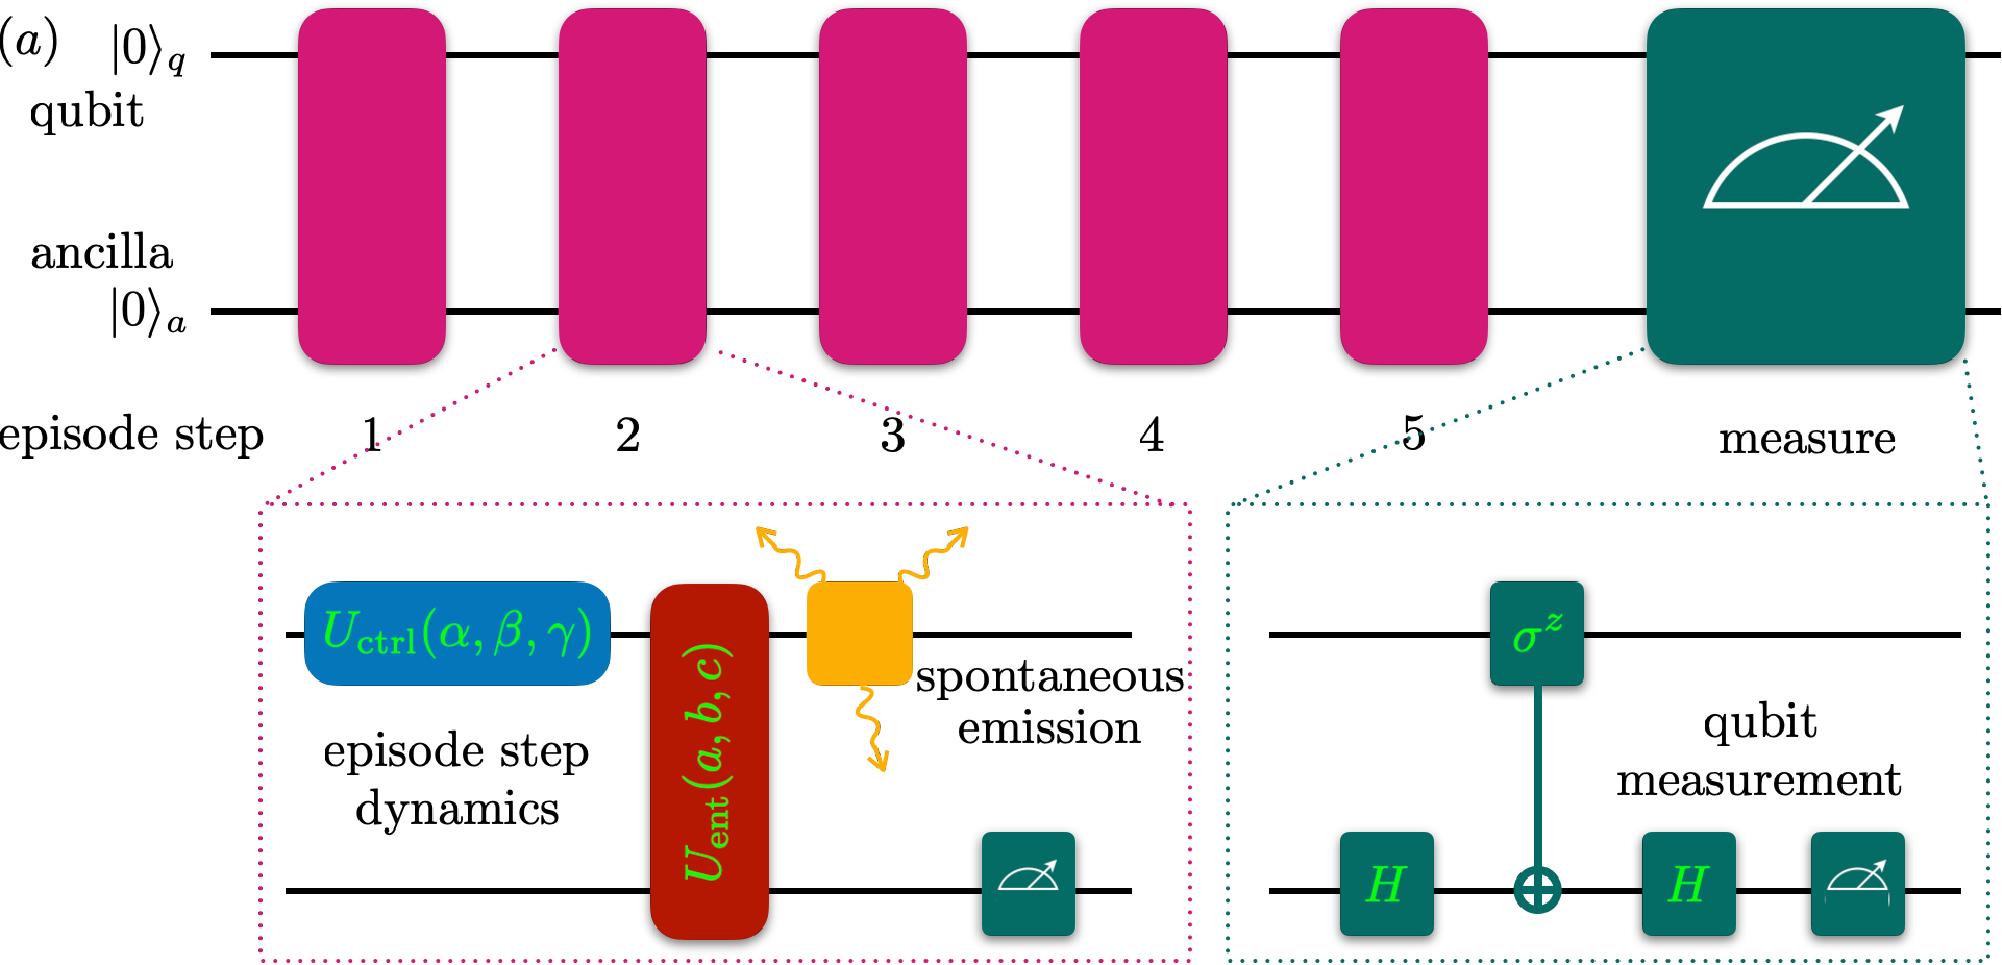
\includegraphics[width=0.58\columnwidth]{RL-qa_schematic.pdf}
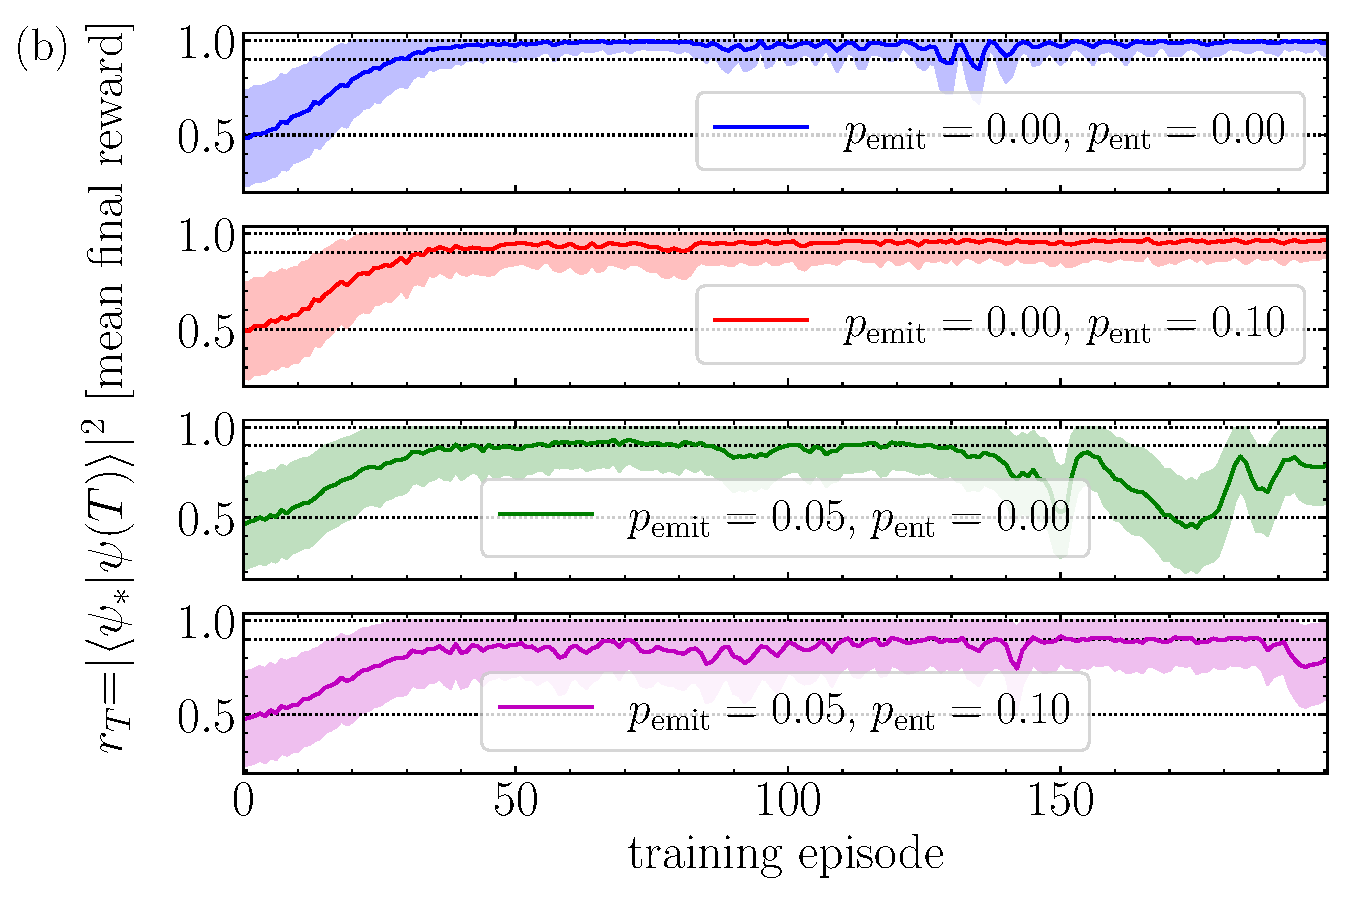
\includegraphics[width=0.41\columnwidth]{RL-qa_training-curve.pdf}
\caption{
Reinforcement learning from quantum data. 
\textbf{(a)} 
We couple a qubit to an ancilla which we can measure projectively. 
At each episode step, the agent can apply a control gate $U_\text{ctrl}(\alpha,\beta,\gamma)$ (blue); however, the system is also subject to entangling noise $U_\text{ent}(a,b,c)$ (red) and spontaneous emission (orange). After each step we project the ancilla on the ground state. The time step, the measurement output, and the detected spontaneously emitted photon represent the RL observations; the reward is given at the end of the circuit by the binary output of the qubit collapse on the target state. At the end of the circuit, we use the ancilla to project the state of the qubit to the target state; this produces a binary output that defines the return.
\textbf{(b)} Training curves showing the final fidelity over a batch of $2048$ trajectories for:
(blue) the clean case (i.e., no entangling noise and no spontaneous emission);
(red) in the presence of entangling noise only; 
(green) in the presence of spontaneous emission only;
(magenta) in the presence of both noise and spontaneous emission. 
%The horizontal dotted lines indicate fidelities of $0.5$, $0.9$, and $1.0$, respectively. 
The shaded area marks the $1\sigma$ window over the batch. 
The horizontal dotted lines mark the $0.5, 0.8, 1.0$ fidelity thresholds, respectively.
We use a single-layer fully-connected neural network with $8$ hidden neurons. 
%\steve{REF COMMENT: In the caption of Fig. 14, at the end the authors state that the horizontal lines indicate fidelities 0.5, 0.9, 1 and immediately below 50\%, 80\%, 100\%. The latter appears to be the correct one.}
}
\label{fig:RL-qdata}
\end{figure}

Figure~\ref{fig:RL-qdata}(a) shows the control protocol applied to the qubit-ancilla system. The purple box represents one step, and is unpacked in the corresponding inset: first, the agent determines the optimal angles $\alpha,\beta,\gamma$ and applies the control unitary; the state then undergoes the entangling noise [blue] (whose strength is random, but fixed during training), followed by an eventual spontaneous emission of the qubit [orange]. Finally, we measure the ancilla in the $z$-basis, and use the binary measurement output as an observation. 
This protocol repeats for a total of $T=5$ steps, before we project the qubit to the target state [green box]. To do so, we use the Hadamard-$C_{\sigma_\ast}$-Hadamard sequence described above: measuring the ancilla in the $z$-basis then returns the correct output (as if we had measured the operator $\sigma_\ast$) and collapses the state of the qubit; it is this measurement data that we use as a reward to train the RL agent. 

We now parameterized the policy by a single-layer fully connected neural network with $8$ hidden neurons; the output of the network are the three mean and standard deviation values; we can sample actions (i.e., angles) from three independent corresponding normal distributions. To train the agent, we use a batch of $2048$ trajectories, over a total of $200$ episodes. Figure~\ref{fig:RL-qdata}(b) shows the corresponding training curves for four different types of noisy environments;
(i) when the entangling noise and spontaneous emission are off ($p_\text{emit}=0$, $p_\text{ent}=0$), the only source of noise is the shot noise when estimating the fidelity. We see that in this case, the agent learns to control the qubit after about $50$ episodes, reaching an almost perfect fidelity. Moreover, the $1\sigma$ uncertainty window (shaded area) shrinks as training progresses which indicates that the policy becomes more deterministic. 
(ii) we can then keep the spontaneous emission off and consider a weak entangling noise. This slightly reduces the achievable final fidelity to about $90\%$, but does not degrade the overall performance of the agent. 
(iii) in the opposite case, with spontaneous emission replacing the weakly entangling gate as a dominant noise source, we find that the agent reaches about $80\%$ fidelity. Following a stable learning stage, we notice large fluctuations in the training curve: these are presumably due to the small neural network used. We expect that training the agent longer will eventually stabilize the curve close to its maximum value.
(iv) finally, we turn all sources of noise on. The overall fidelity achieved by the agent in this case lies at around $80\%$. 
We invite the interested reader to check out the accompanying Jupyter notebook and explore the behavior of the agent further~\cite{github_code}.

\steve{Generalizing this setup beyond single-qubit control is a topic of forefront research. For instance, there was a recent demonstration of how RL agents can discover error-correcting codes in few-qubit systems by using an ancilla to infer partial information about the state of the system~\cite{foesel2018reinforcement}. 
Similarly, a recent experimental realization of a GKP code built from the states of a cavity resonator and manipulated using a transmon qubit as an ancilla~\cite{sivak2023real}, provides another real-world application of the framework introduced above. For details, we refer the interested readers to the growing body of literature on using RL for quantum error correction. 
}

\subsection{\label{subsec:RL_exp}Implementations of reinforcement learning in experiment}

We close this section by mentioning three applications of RL in experiments with quantum systems. The field is rapidly evolving; hence, the selection below is to be taken as exemplary rather than exhaustive. 

%%%%%%%%%%%%%%%%%%%%%%%%%%%%

In Ref.~\cite{reuer2023realizing} the authors used an RL agent to initialize the state of a single transmon qubit. This state preparation task requires real-time control on time scales much shorter than the coherence time of a qubit. Thus, for the purpose of efficiency, the RL agent has to be integrated with the experimental device requiring low-latency feedback. The authors achieved this by using a sub-microsecond-latency neural network on a field-programmable gate array (FPGA) which interacts directly with the transmon qubit. The agent was then trained using quantum measurements. 
This work laid the foundations for resolving the challenge of developing and training a reinforcement learning agent able to operate using real-time feedback.


%%%%%%%%%%%%%%%%%%%%%%%%%%%%



A more difficult, yet closely related, problem is the preparation of quantum gates. Quantum gates are implemented using control pulses, much like those discussed in Sec.~\ref{sec:QOC}. Gate synthesis can be viewed as a state preparation problem, but for a collection of a complete basis set for the Hilbert space; the challenge is to prepare the basis states with the correct relative phases among them. The agent typically has access to the control fields of a Hamiltonian, the time evolution of which generates the quantum gate.
RL has proven useful in tasks involving the design of low-level pulse controls that can compensate for hardware errors. In Ref.~\cite{baum2021experimental}, the authors demonstrate an RL agent that can design a universal set of error-robust quantum logic gates. In particular, they also train their agent in runtime on a superconducting quantum computer to implement a cross-resonance two-qubit gate. The agent does not require knowledge of a Hamiltonian model for the system, its controls, or any underlying error processes. The pulse sequences produced by the RL agent for the cross-resonance gate are up to three times faster than state-of-the-art pulses. Moreover, RL gates were found to be robust against calibration drifts.




% Most studies focus on finding better single- and two-qubit gates for quantum computing in the presence of various known and unknown sources of noise. 

% For instance, in Ref.~[CITE], the authors used PG to improve theoretical optimal control pulses for a cross-resonance gate on a transmon qubit device in the presence of noise. They deployed their agent on an IBM machine and achieved an almost order-of-magnitude improvement in gate fidelities. 


% Recently, Ref.~[CITE] trained a DDPG agent in a simulator to find entangling gates without any previous bias, and showed an improvement of one order of magnitude and a reduction in the gate duration. The learning capabilities of the agent allow it to be trained for varying system parameters (e.g., transmon frequency, anharmonicity, coupling, drive strength, etc.) making the pulses it yields resilient to small changes and drifts with time. 

%%%%%%%%%%%%%%%%%%%%%%%%%%%%

%A third class of application of RL to quantum technologies is the construction of variational quantum circuits. A quantum circuit is a sequence of gates, that provide the basics to execute operations on digital quantum computing devices. Since gates are represented by unitary operators, in general, they do not commute. Thus, given a set of gates, the question arises as to what the optimal order of placing the gates is, to implement a given target operation in a circuit. As in practice gates are typically prone to errors, optimality here often refers to reducing the number of gates in the circuit [CITE], which leads to a discrete combinatorial optimization problem. In other cases, where the structure of the circuit is fixed, optimality may also refer to finding the best values for a set of continuous parameters that define each elementary gate operation [CITE]. When considering applications of RL for the optimization of quantum circuits, one should pay specific attention to the interface between the agent and the NISQ device. 

%%%%%%%%%%%%%%%%%%%%%%%%%%%%

And finally, a generalization of the RL framework used in Sec.~\ref{subsec:RL_qubit_ancilla} was recently used in an experiment to demonstrate quantum error correction for a cavity-QED qubit. The cavity mode defines a harmonic oscillator from which a logical qubit is built using a Gottesman-Kitaev-Preskill (GKP) code. The oscillator is coupled to a transmon which allows for readout and control of the logical qubit. The RL agent is trained to preserve the logical subspace using measurements of the code stabilizers. As a result, the trained RL agent increases the lifetime of the GKP qubit by more than a factor of 2, using an active quantum error correction protocol~\cite{sivak2023real}.


%Quantum error correction (QEC) provides yet another notable set of problems for RL. In the context of stabilizer codes, one considers a (large) number of interacting physical qubits that encode a single logical qubit in a subspace of their Hilbert space. If the logical states are entangled superpositions of the computational states of the physical qubits (as in the case of the topological surface code), this serves to protect the logical qubit states against decoherence. When a bit- or a phase-flip error occurs in a physical qubit, a stabilizer measurement returns an error syndrome. Using the information in the syndrome measurement, one can apply a recovery operation to bring the state back to the logical qubit manifold. However, as it happens, the same error can give rise to different syndromes, and thus the optimal recovery operation is a priori unclear. Moreover, since errors occur probabilistically, the recovery model should also be probabilistic. In the context of QEC, RL agents observe syndrome measurements, and try to correct the underlying error. Recent work has demonstrated that RL agents can perform on par with state-of-the-art error correction algorithms [CITE].